\documentclass[bibliography=totocnumbered]{scrartcl}
\usepackage{imakeidx}
\usepackage{ragged2e}
\usepackage{setspace} % Um den Zeilenabstand zu ändern.
\usepackage{gensymb}
%\usepackage{authblk}
% \usepackage{minitoc} % for the chpaters
\usepackage{wasysym}
%\usepackage{SI}
\usepackage{array} % Verwendung von Matrizen
\usepackage{booktabs} % Schöne Tabellen beziehungsweise sie sehen damit professioneller aus.
\usepackage{tabulary} % Ähnlich wie tabularx, ermöglicht aber das ändern der Ausrichtung der Spalten.
\usepackage{tabularx} % Tabellen mit automatischen Zeilenumbruch.
\usepackage{enumitem}
\usepackage{physics}
\usepackage[T1]{fontenc}% fontec und inputenc ermöglichen
\usepackage{graphicx}%Für Grafiken
\usepackage{rotating} % lässt Grafiken rotieren
\usepackage{mathtools}% mathematische Werkzeuge
\usepackage{amsmath}% Mathetools
\usepackage{amsfonts}% Mathetools
\usepackage{amssymb}% Symbole wie Natürliche Zahlen
\usepackage{geometry}
%\usepackage{bibtex} 
\usepackage{tablefootnote}% Fußnoten in Tabellen
\usepackage{float}% für eingebundene Bilder
\usepackage{fancyhdr} % Seiten schöner gestalten, insbesondere Kopf- und Fußzeile
\usepackage{ulem} 
\usepackage{dcolumn}% Align table columns on decimal point
\usepackage{bm}% bold math
\usepackage[ngerman]{babel} % Worttrennung nach der neuen Rechtschreibung und deutsche Bezeichnungen. babelfunktion wird wegen Literatur gebraucht.
\usepackage{subfloat} % Was macht diese Packet?
\usepackage{caption} % Unter-/Überschriften für Bilder, Grafiken und Tabellen
\usepackage{subcaption}
\usepackage{txfonts}
\usepackage{titling}% Titel
\usepackage[style=alphabetic]{biblatex} %biblatex mit alphabetic laden. alphbetic=Zitationsstil
\usepackage{bookmark}
\usepackage[printonlyused]{acronym}
\usepackage{amsthm}
\usepackage{pdfpages}
\usepackage{tikz}
\usepackage[siunitx,americanvoltages, europeanresistors,americancurrents]{circuitikz}
\usepackage{listings}
\usepackage{abstract}
\usepackage[per-mode = fraction]{siunitx}
\usepackage{hyperref}
\newcommand{\R}{\mathbb{R}} % reelle Zahlen
\newcommand{\N}{\mathbb{N}} % natürliche Zahlen
\newcommand{\C}{\mathbb{C}} % komplexe Zahlen
\newcommand{\Q}{\mathbb{Q}} % rationale Zahlen
\newcommand{\Z}{\mathbb{Z}} % ganze Zahlen
\newcommand{\F}{\mathbf{F}} % Kraft
\newcommand{\E}{\mathbf{E}} % Energie
\newcommand{\V}{\mathbf{v}} % Geschwindigkeit
\newcommand{\B}{\mathbf{B}} % magnetischer Fluss
\newcommand{\J}{\mathbf{j}} % Stromdichte ?
\newcommand{\D}{\mathbf{D}} % elektrische Induktion
\newcommand{\HH}{\mathbf{H}} % magnetische Feldstärke
\newcommand{\M}{\mathbf{M}} % Magnetisierung
\newcommand{\p}{\mathbf{P}}
\newcommand{\rr}{\mathbf{r}}
\newcommand{\vp}{\varphi}
\newcommand{\ve}{\varepsilon}
\newcommand{\vcc}[1]{\left(\begin{matrix}#1\end{matrix}  \right)}
\newcommand{\m}[1]{\left\lbrace #1\right\rbrace}
\newcommand{\los}{\noindent\textbf{Lösung}:}
\newcommand{\rang}[2]{\text{Rang}(#1)=#2}
\newcommand{\vpe}{\frac{1}{4\pi\ve_0}}
\newcommand{\qvpe}{\frac{q}{4\pi\ve_0}}
\newcommand{\geg}{\ac{geg.}}
\newcommand{\ges}{\ac{ges.}}

\newcommand{\kommando}[1]{$\backslash$\textit{#1}}
\newcommand{\com}[1]{$\backslash$\textit{#1}$\left\lbrace\ldots\right\rbrace$}
\newcommand{\Com}[2]{$\backslash$\textit{#1}$\left\lbrace #2\right\rbrace$}
\newcommand{\NeuKommando}[2]{$\backslash \textit{#1} \left\lbrace \backslash \textit{#2}\right\rbrace$}
\newcommand{\latex}{\LaTeX $\;$}


% si unitx
\DeclareSIUnit\litre{l}

\hypersetup{
	colorlinks=true,
	linkcolor=blue,
	filecolor=magenta,      
	urlcolor=cyan,
	citecolor=lime!50!black,
	filecolor=red
}
%\addbibresource{} %Bibliographiedateien laden
\addbibresource{bib.bib}

\geometry{a4paper, left=25mm, right=25mm, top=30mm, bottom=30mm}
\lhead{\thedate}
\rhead{GPR}
\lhead{\thetitle}
\pagestyle{fancy}

\usetikzlibrary{patterns}
\usetikzlibrary{3d}
\makeindex[title=Stichwortverzeichnis,intoc
,options= -s Index-Formatierung.ist
]
\author{Ben J. F.}
\allowdisplaybreaks

\lstset
{ %Formatting for code in appendix
    basicstyle=\footnotesize,
    numbers=left,
    stepnumber=1,
    showstringspaces=false,
    tabsize=2,
    breaklines=true,
    breakatwhitespace=false,
}

\date{19.05.2021}

\title{T7 \\Spezifische Wärmekapazität idealer Gase}


\rfoot{T7}

\begin{document}
	\newgeometry{left=14mm, right=13.5mm, top=60mm, bottom=30mm}
	\begin{titlepage}
		\begin{center}
			{\huge{Grundpraktikum}}\\\vspace*{15mm}
			{\huge{\textbf{\thetitle}}}\\\vspace*{20mm}
			{\theauthor}\\\vspace*{10mm}
			{\thedate}\\\vspace*{40mm}
			
			
			
			
		\end{center}
	\end{titlepage}
	\makeatother
	\restoregeometry
	\newpage
	
	\tableofcontents
    \newpage
	\listoffigures 
	\listoftables
	\newpage
	\section{Einleitung}
	Motivation des Versuchs ist die Bestimmung der Adiabatenexponenten $ \kappa $ von Luft und Argon zu bestimmen. Dafür werden Messungen einer adiabatischen Expansion genutzt, dies geschieht unter Annahme des idealen Gases. Diese ist abhängig von dem atomaren Aufbau der Moleküle. \\
	Theoretische Herleitungen und wieter Inforamtionen wird im Skript \smartcite[vgl][1f]{T7} erklärt.
	\section{Versuchsaufgbau}
	Das Experiment wird in 2 verschiedene Experimente unterteilt.
	\subsection{$\kappa$-Bestimmung nach Clément-Desormes}
	Hier wird mittels eines Druckballes der Druck in einer luftgefüllten Glasflasche, mit ca. 20l Fassungsvermögen, erhöht. Anschließend öffnet man einen Zweigarm, so dass Außenluft reinströmen kann, so kommt es zu einem adiabatischen Druckausgleich. Schließt man die Luftzufuhr, so steigt die Temperatur wieder auf die Umgebungstemperatur an, da es durch den adiabatische Druckausgleich zu einer Temperatursenkung gekommen ist. Dadurch kommt es zum Druckanstieg. Dieser wird gemessen anhand des Manometers. In Material (\cite{T7}) wird hergeleitet, dass für den Adiabatenexponenten gilt:
	\begin{equation}\label{eq: kappa eq Desormes}
		\kappa = \dfrac{h_{1}}{h_{1}-h_{2}}
	\end{equation}
	Wobei $ h_{1} $ die Höhendifferenz beim Manometer ist vor dem Öffnen des Zweigarms und $ h_{2} $ die nach dem Öffnen. Da durch Änderung der Zimmertemperatur, der Überdruck nicht konstant ist, sondern linear steigt, soll man 5 Minuten nahc und vor der Expansion die Höhendifferenz am Manometer ablesen und als Korrekturverfahren nutzen.
	\subsection{$\kappa$-Bestimmung nach Rückhardt}
	In diesem Experiment  soll der Exponent bestimmt werden durch die Schwingung durch die Gasleitung. Hier ist in einem Glaskolben (mit Volumen V) das zu untersuchende Gas eingeleitet. Auf den Glaskolben ist ein Rohr, der Länge $ l $ und Radius $ r $, mit einer Öffnung in der Mitte. Anschließend wird ein Körper, der Masse $ m_{1} $, eingeführt. Durch den Druck, der durch das einströmende Gas entsteht, wird der Schwingkörper nach oben beschleunigt, ist dieser jedoch über der Öffnung, so kommt es zu einem Druckabfall und die Schwerkraft wirkt. Somit kommt es zu einer nahezu ungedämpften Schwingung, da die Energie durch das Glas, der Reibung entgegen wirkt. Aus dem Versuchsskript (\cite{T7}) folgt:
	\begin{equation}\label{eq: kappa eq Rückhardt}
		\kappa= \dfrac{4Vm}{r^{4}p T^{2}}
	\end{equation}
	Wobei $p $ der Druck in der Flasche, T die Periodendauer der Schwingung und $ m $ die schwingende Masse bezeichnet. Weitere Informationen, genauere Beschreibungen und Herleitungen der Gleichungen sind im Skript (\cite{T7}) zu finden.
	
	\newpage
	\section{Versuch 1}
    \begin{table}[H]
        \centering
		\caption{gemessener Temperatur und Außendruck}
		\begin{tabular}{|c|c|}
			\hline
			Temperatur   & Außendruck \\
			%\hline
			$\left[\text{Grad}\right]$ & $\left[\text{kPa}\right]$ \\
			\hline
			22.5  & 100 \\
			\hline
			23 & 99.8 \\
			\hline
		\end{tabular}
	\label{tab: Temp und A.druck}
    \end{table}
	
	Hier wurden 4 mal die adiabatische Expansion gemessen, unter Temperatur und Außendruck in der ersten Zeile aus Tabelle (\ref{tab: Temp und A.druck}) und 4 mal wurde die adiabatische Expansion mit der zweiten Zeile aus Tabelle (\ref{tab: Temp und A.druck}) gemessen.
	 Da durch Änderung der Zimmertemperatur, der Überdruck nicht konstant ist, sondern linear steigt, soll man 5 min nach und vor der Expansion die Höhendifferenz am Manometer ablesen und als Korrektur verfahren nutzen. \\
	 Daraus ergeben sich die Graphen aus der Abb. (\ref{Abb: Ben 1}), Abb. (\ref{Abb: Ben 2}), Abb. (\ref{Abb: Ben 3}), Abb. (\ref{Abb: Ben 4}), Abb. (\ref{Abb: Sara 1}), Abb. (\ref{Abb: Sara 2}),Abb. (\ref{Abb: Sara 3}) und Abb. (\ref{Abb: Sara 4}).\\
	 Daraus ergeben sich die folgenden Adiabatenexponenten nach der Formel (\ref{eq: kappa eq Desormes}):
	 \begin{table}[ht!]
	\centering
	\caption{Ergebnisse zum Adiabatenexponten nach Clément-Desormes}
	 	\begin{tabular}{|c|c|c|}
	 		\hline
	 		$\kappa$-Nummerierung & Experimentatorin & Experimentator \\
	 		\hline
	 		1 & 1.28 & 1.11 \\
	 		\hline
	 		2 & 1.37 & 1.17 \\
	 		\hline
	 		3 & 1.16 & 1.13 \\
	 		\hline
	 		4 & 1.07 & 1.31 \\
	 		\hline
	 	\end{tabular}
 	\label{tab: kappa nach Clément}
	 \end{table}
 
	  Durch die Gaußsche Fehlerfortpflanzung kann man die Unsicherheiten bestimmen.
	  \begin{equation}\label{eq: Unsicherheit h}
	  	u_{h_{1}}=u_{h_{2}}=\sqrt{u_{h_{1}}^{2}+u_{h_{2}}^{2}}=u_{h}\sqrt{2}
	  \end{equation}
	 \begin{equation}\label{eq: Unsicherheit kappa}
	 	u_{k}=\dfrac{1}{\Delta h}\sqrt{\left(u_{hp_{1}}h_{p_{2}}\right)^{2}+\left(u_{hp_{2}}h_{p_{1}}\right)^{2}}
	 \end{equation}
 Als gewichtetes Mittel der Adiabatengleichung ergibt sich dann der Wert 1.20.
	
	
	
	\newpage
	\section{Versuch 2}
	Für das Experiment wurde für den Kolben und das Rohr, der Radius $ R=(6.965\pm 0.005) $ mm, der Länge $ l=(19.30\pm 0.07) $cm,
	 dem Volumen $ V=(4381\pm 10) $ cm$ ^{3} $.
	Die Masse hatte die Masse $ m_{1}=(6.122\pm0.005) $g.
	Am Barometer wurde der Außendrücke $ p_{0}=99.5 $kPa und $ p_{0}=100 $kPa  und die Temperaturen $ T=294.15 $Kelvin und $ T=295.65 $ gemessen.
	Es wurden die Periodendauer für 100 Schwingungen nun gemessen:
	\begin{table}[ht!]
		\centering
		\caption{Messergebnisse der Periodendauer über 100 Schwingungen von der Experimenatorin und vom Experimentator für Luft}
		\begin{tabular}{|c|c|c|}
			\hline
			Messung & Experimentatorin & Experimentator \\
			\hline
			1 & 58.26 & 57.74 \\
			\hline
			2 & 58.22 & 57.66 \\
			\hline
			3 & 58.21 & 57.66 \\
			\hline
			4 & 58.21 & 57.64 \\
			\hline
			5 & 58.20 & 57.65 \\
			\hline
			6 & 58.17 & 57.65 \\
			\hline
		\end{tabular}
		\label{tab: M.ergebnisse A2 T100}
	\end{table}
	Um den adiabatischen Exponenten zu bestimmen müssen wir vorher noch folgendes berechnen.Die schwingende Masse ist die Summe aus der Masse des Körpers und der des Gases, dass mit schwingt.Die Masse des Gases kann man durch die Relation von Masse zu Volumen bestimmen.Dabei ist bei der bekannter Dichte der Luft …:
	
	\begin{align}\label{eq: m2}
		m_{2,S.R.}=\rho V=\rho \pi r^{2}l=4.7\cdot 10^{-5} \text{ kg}\\
		m_{2,B.F.}=\rho V=\rho \pi r^{2}l=4.4 \cdot10^{-5} \text{ kg}
	\end{align}
\begin{align}\label{eq: Unsicherheit von m2}
	u_{m_{2},S.R.}=\rho \pi \sqrt{ \left(2u_{r}lr\right)^{2}+\left(u_{l}r^{2}\right)^{2}}=0.0008\text{ kg}\\
	u_{m_{2},B.F.}=\rho \pi \sqrt{ \left(2u_{r}lr\right)^{2}+\left(u_{l}r^{2}\right)^{2}}=0.0008\text{ kg}
\end{align}
Damit ergibt sich für die Gesamtmasse:
\begin{align}\label{eq: Gesamtmasse}
	m_{S.R}=m_{1}+m_{2}=6.169\cdot 10 ^{-3}\text{ kg}\\
	m_{B.F}=m_{1}+m_{2}=6.166\cdot 10 ^{-3}\text{ kg}
\end{align}
\begin{equation}\label{eq: Unischerheit von Gesamtmasse}
	u_{m}=\sqrt{u_{m_{1}}^{2}+u_{m_{2}}^{2}}=9\cdot 10 ^{-4}\text{ kg}
\end{equation}
	Nun gilt es ebenso der Druck in der Falsche zu bestimmen, den bestimmt man durch die Formel:
	\begin{align}
		p_{S.R}=p_{0}+\dfrac{mg}{\pi r^{2}}=99894.07 \text{Pa}\\
		p_{B.F}=p_{0}+\dfrac{mg}{\pi r^{2}}=100394.07 \text{Pa}\\
		u_{p}=\sqrt{u_{p_{0}}^{2}+\left(\dfrac{u_{m}g}{\pi r^{2}}\right)^{2}+\left(\dfrac{2u_{r}mg}{\pi r^{3}}\right)^{2}}
	\end{align}
	Da für die Periodendauer gilt:
	\begin{align}
		T=\dfrac{t}{100}\\
		u_{T}=\dfrac{u_{T}}{\sqrt{600}}
	\end{align}
	Durch die Formeln 2 und 5 bis 16 ergeben sich nun die adiabatischen Exponenten:
	
	\begin{table}[ht!]
		\centering
		\caption{$\kappa$-Ergebnisse aus dem Versuch 2}
		\begin{tabular}{|c|c|}
			\hline
			Experimentatorin  & Experimentator \\
			\hline
			1.366$ \pm $0.014& 1.362$ \pm $0.014 \\
			\hline
			1.368$ \pm $0.014 & 1.366$ \pm $0.014 \\
			\hline
			1.368$ \pm $0.014 & 1.366$ \pm $0.014 \\
			\hline
			1.368$ \pm $0.014 & 1.367$ \pm $0.014 \\
			\hline
			1.368$ \pm $0.014 & 1.366$ \pm $0.014 \\
			\hline
			1.370$ \pm $0.014 & 1.366$ \pm $0.014 \\
			\hline
		\end{tabular}
		\label{tab: kappa V2}
	\end{table}
	
	Mit der Unsicherheit
	\begin{equation}\label{eq: Unsicherheit von Kappa V2}
		u_{k}=\sqrt{\dfrac{u_{m}^{2}}{m^{2}}+\dfrac{u_{V}^{2}}{V^{2}}+\dfrac{4u_{r}^{2}}{r^{2}}+\dfrac{2u_{T}^{2}}{T^{2}}+\dfrac{u_{p}^{2}}{p^{2}}}
	\end{equation}
	Es ergibt sich nun das gewichtete Mitte von $ \kappa $:\\
	- Experimentatorin: $ 1.37\pm 0.03 $\\
	- Experimentator: $ 1.37\pm 0.03 $
	
	
	
	\newpage
	\section{Versuch 3}
	Für das Experiment wurde für den Kolben und das Rohr, der Radius $ R=(6.975\pm 0.005) $ mm, der Länge $ l=(18.0\pm 0.3) $cm und dem Volumen $ V=4325\pm 10 $cm$ ^{3} $.
	Die Masse hatte die Masse $ m_{1}=(6.231\pm 0.005) $g.
	m Barometer wurde der Außendrücke $ p_{0}=99.5 $kPa und $ p_{0}=100 $kPa  und die Temperaturen $ T=294.15 $Kelvin und $ T=295.65 $ gemessen.
	Es wurden die Periodendauer für 100 Schwingungen nun gemessen:
	
	\begin{table}[ht!]
		\centering
		\caption{Messergebnisse der Periodendauer über 100 Schwingungen von der Experimenatorin und vom Experimentator für Argon}
		\begin{tabular}{|c|c|c|}
			\hline
			Messung & Experimentatorin & Experimentator \\
			\hline
			1 & 53.63 & 53.56 \\
			\hline
			2 & 53.61 & 53.52 \\
			\hline
			3 & 53.60 & 53.54 \\
			\hline
			4 & 53.59 & 53.54 \\
			\hline
			5 & 53.59 & 53.58 \\
			\hline
			6 & 53.59 & 53.59 \\
			\hline
		\end{tabular}
		\label{tab: M.ergebnisse A3 T100}
	\end{table}
	Durch die Formeln 2 und 5 bis 16 ergeben sich nun die adiabatischen Exponenten:\\
	\begin{equation}\label{eq: Masse 2 Argon}
		m_{2}=7.9\cdot 10^{-5}
	\end{equation}
\begin{align}\label{eq: Druck}
	p_{S.R}=100199.93\text{Pa}\\
	p_{B.F}=100399.93\text{Pa}
\end{align}
	Als adiabatischer Exponent ergibt sich:\\
	\begin{table}[ht!]
		\centering
		\caption{$\kappa$-Ergebnisse aus dem Versuch 3}
		\begin{tabular}{|c|c|}
			\hline
			Experimentatorin  & Experimentator \\
			\hline
			1.649$ \pm $0.017& 1.631$ \pm $0.017 \\
			\hline
			1.650$ \pm $0.017 & 1.634$ \pm $0.017 \\
			\hline
			1.650$ \pm $0.017 & 1.633$ \pm $0.017 \\
			\hline
			1.651$ \pm $0.017 & 1.633$ \pm $0.017 \\
			\hline
			1.651$ \pm $0.017 & 1.630$ \pm $0.017 \\
			\hline
			1.651$ \pm $0.017 & 1.630$ \pm $0.017 \\
			\hline
		\end{tabular}
		\label{tab: kappa V3}
	\end{table}
	
	E gibt sich nun das gewichtete Mittel von $\kappa$ :
	- Experimentatorin: 1.65$\pm$0.04\\
	- Experimentator: 1.63$\pm$0.04
	\newpage
	\section{Vergleich }
	Da Luft größtenteils aus dreiatomigen Stoffen besteht (Stickstoff, Sauerstoff, Wasser…) kann man als Idealwert des Adiabatenexponenten, die für Atome des Freiheitsgrades 3 nehmen, also 1.33
	Für Argon gilt der Freiheitsgrad 1, somit 1.66
	Die Werte des zweiten und dritten Versuches sind sehr dicht an diesem, währen die des ersten Experimentes markant geringer ist, was durch die Temperaturkorrektur entsteht. Ebenso scheint es kaum einen Anstieg zu geben.Ohne die Korrektur, würden folgende Werte entstehen.
	Jedenfalls sieht man, dass Exp 2 und 3 genauere Ergebnisse liefern und näher am theoretischen Wert ist.
	
	
	\section{Fehlerquellen}
	\subsection{Waagerechtes Ablesen/Oberflächenspannung}
	Im Versuch 1 bei den Messreihen war es für die Experimentatorin Aufgrund ihrer Körpergröße sehr erschwert, den Wert genau abzulesen, dies sorgt natürlich für eine größere Unsicherheit der Werte für den Anstieg. Für die Experimentatoren waren durch die Oberflächenspannung der Flüssigkeit im Versuch 1 ein korregtes Ablesen erschwert worden. Deswegen hat sich der Experimentator sich dazu entschieden eine Fehlerabschätzung von 2mm vorzunehmen, welche in die Abbildungen (\ref{Abb: Ben 1}), (\ref{Abb: Ben 2}), (\ref{Abb: Ben 3}) und (\ref{Abb: Ben 4}) mit eingeflossen sind.\\
	\subsection{Schneller Ausgleich der Temperatur}
	Man bemerkt, dass sich vor der Expansion schnell ein konstanten Druck gibt, was bedeutet, dass es schnell zu einem Temperaturausgleich kommt, darum ist vor der Expansion die Steigung kleiner als nach der Expansion.
	Vergeringeres Volumen\\
	\subsection{Veringertes Volumen}
	Bei dem RüchardtExperiment strömt Gas aus der Öffnung des Rohres, somit weniger Gasmasse bewegt wird, somit entsteht ein kleinerer Wert für den Adiabatenexponenten, als tatsächlich entstanden ist.\\
	\subsection{Temperaturen}
	Besonders bei dem Experiment von Rüchard, war das Experiment in der Nähe des Fensters aufgebaut, somit ist die Temperatur geringer, als die bei der Tür gemessenen Raumtempertur. Ebenso entstehen weitere Schwankungen der Luft, was den Druck leicht beinflusst.
	Annahme konstanter/fehlerfreier Dichte\\
	\subsection{Annahme konstanter/fehlerfreier Dichte}
	Die Dichte variiert minimal durch die Temperatur. Somit ist die Dichte nicht konstant und oder Fehlerfrei. Dies würde zu einem größeren Fehler führen für den Rüchardt Versuch.
	Reibung\\
	\subsection{Reibung}
	Bei einem Nebenexperiment, wo man bestimmte, bei gekappter Luftzufuhr, wann die Reibung zu groß ist, so dass es keine Schwingung mehr gibt.
	Bei Luft waren es 66 und bei Argon 148 Schwingungen.Dies bedeutet, dass bei Argon die Reibung vollkommen vernachlässigbar.Bei Luft hat sie durch den Luftstrom, die der Reibung entgegenwirkt, somit kann man diese auch vernachlässigen.\\
	
	\subsection{Ideales Gas}
	Es wurde angenommen, dass wir ein ideales Gas haben, was jedoch eine ideelle Vorstellung ist, da nur die Edelgase von den Eigenschaften nahe dem idealen Gasen sind.Doch ist dies vernachlässigbar, da die Reibung kaum einen Einfluss ausübt und Luft annährend als ideales Gas angenommen werden kann
	
	\section{Schlussfolgerung}
	Im Experiment 2 und 3 kann man nicht viel ändern, da man für die Dichte den Druck bräuchte, für die man die Gasmasse bräuchte, was mit der Dichte zusammen hängt.
	Bei dem Clément-Desormes Versuch scheint die Temperaturkorrektur, jedoch eher den Wert zu verschlechtern, sei es wegen ungenauem Messen oder zu schnellen Temperaturausgleich.Jedenfalls sollte davon in zukünftigen Experimenten abgesehen werden, da dies Zeit kostet und durch fast konstanter Raumtemperatur kaum einen Einfluss hat.
	Sinnvoller und genauere Werte würde es geben, wenn man ohne die Korrektur eine oder zwei Minuten, nach der Expansion, die Höhendifferenz misst und anschließend den Durchschnitt berechnet, dies würde zeitsparender sein und genauere Werte liefern.Außerdem würde es sinnvoll sein den Clément-Desormes Versuch mit mehreren Volumen zu widerholen, um die Abhängigkeit von dem Volumen zur Differenz zu sehen.
	\newpage
     \appendix
	\section{Anhang}
	
	\subsection{Temperaturkorrekturen}
	\begin{figure}[!ht]
		\centering									% Bild Zentrierung
		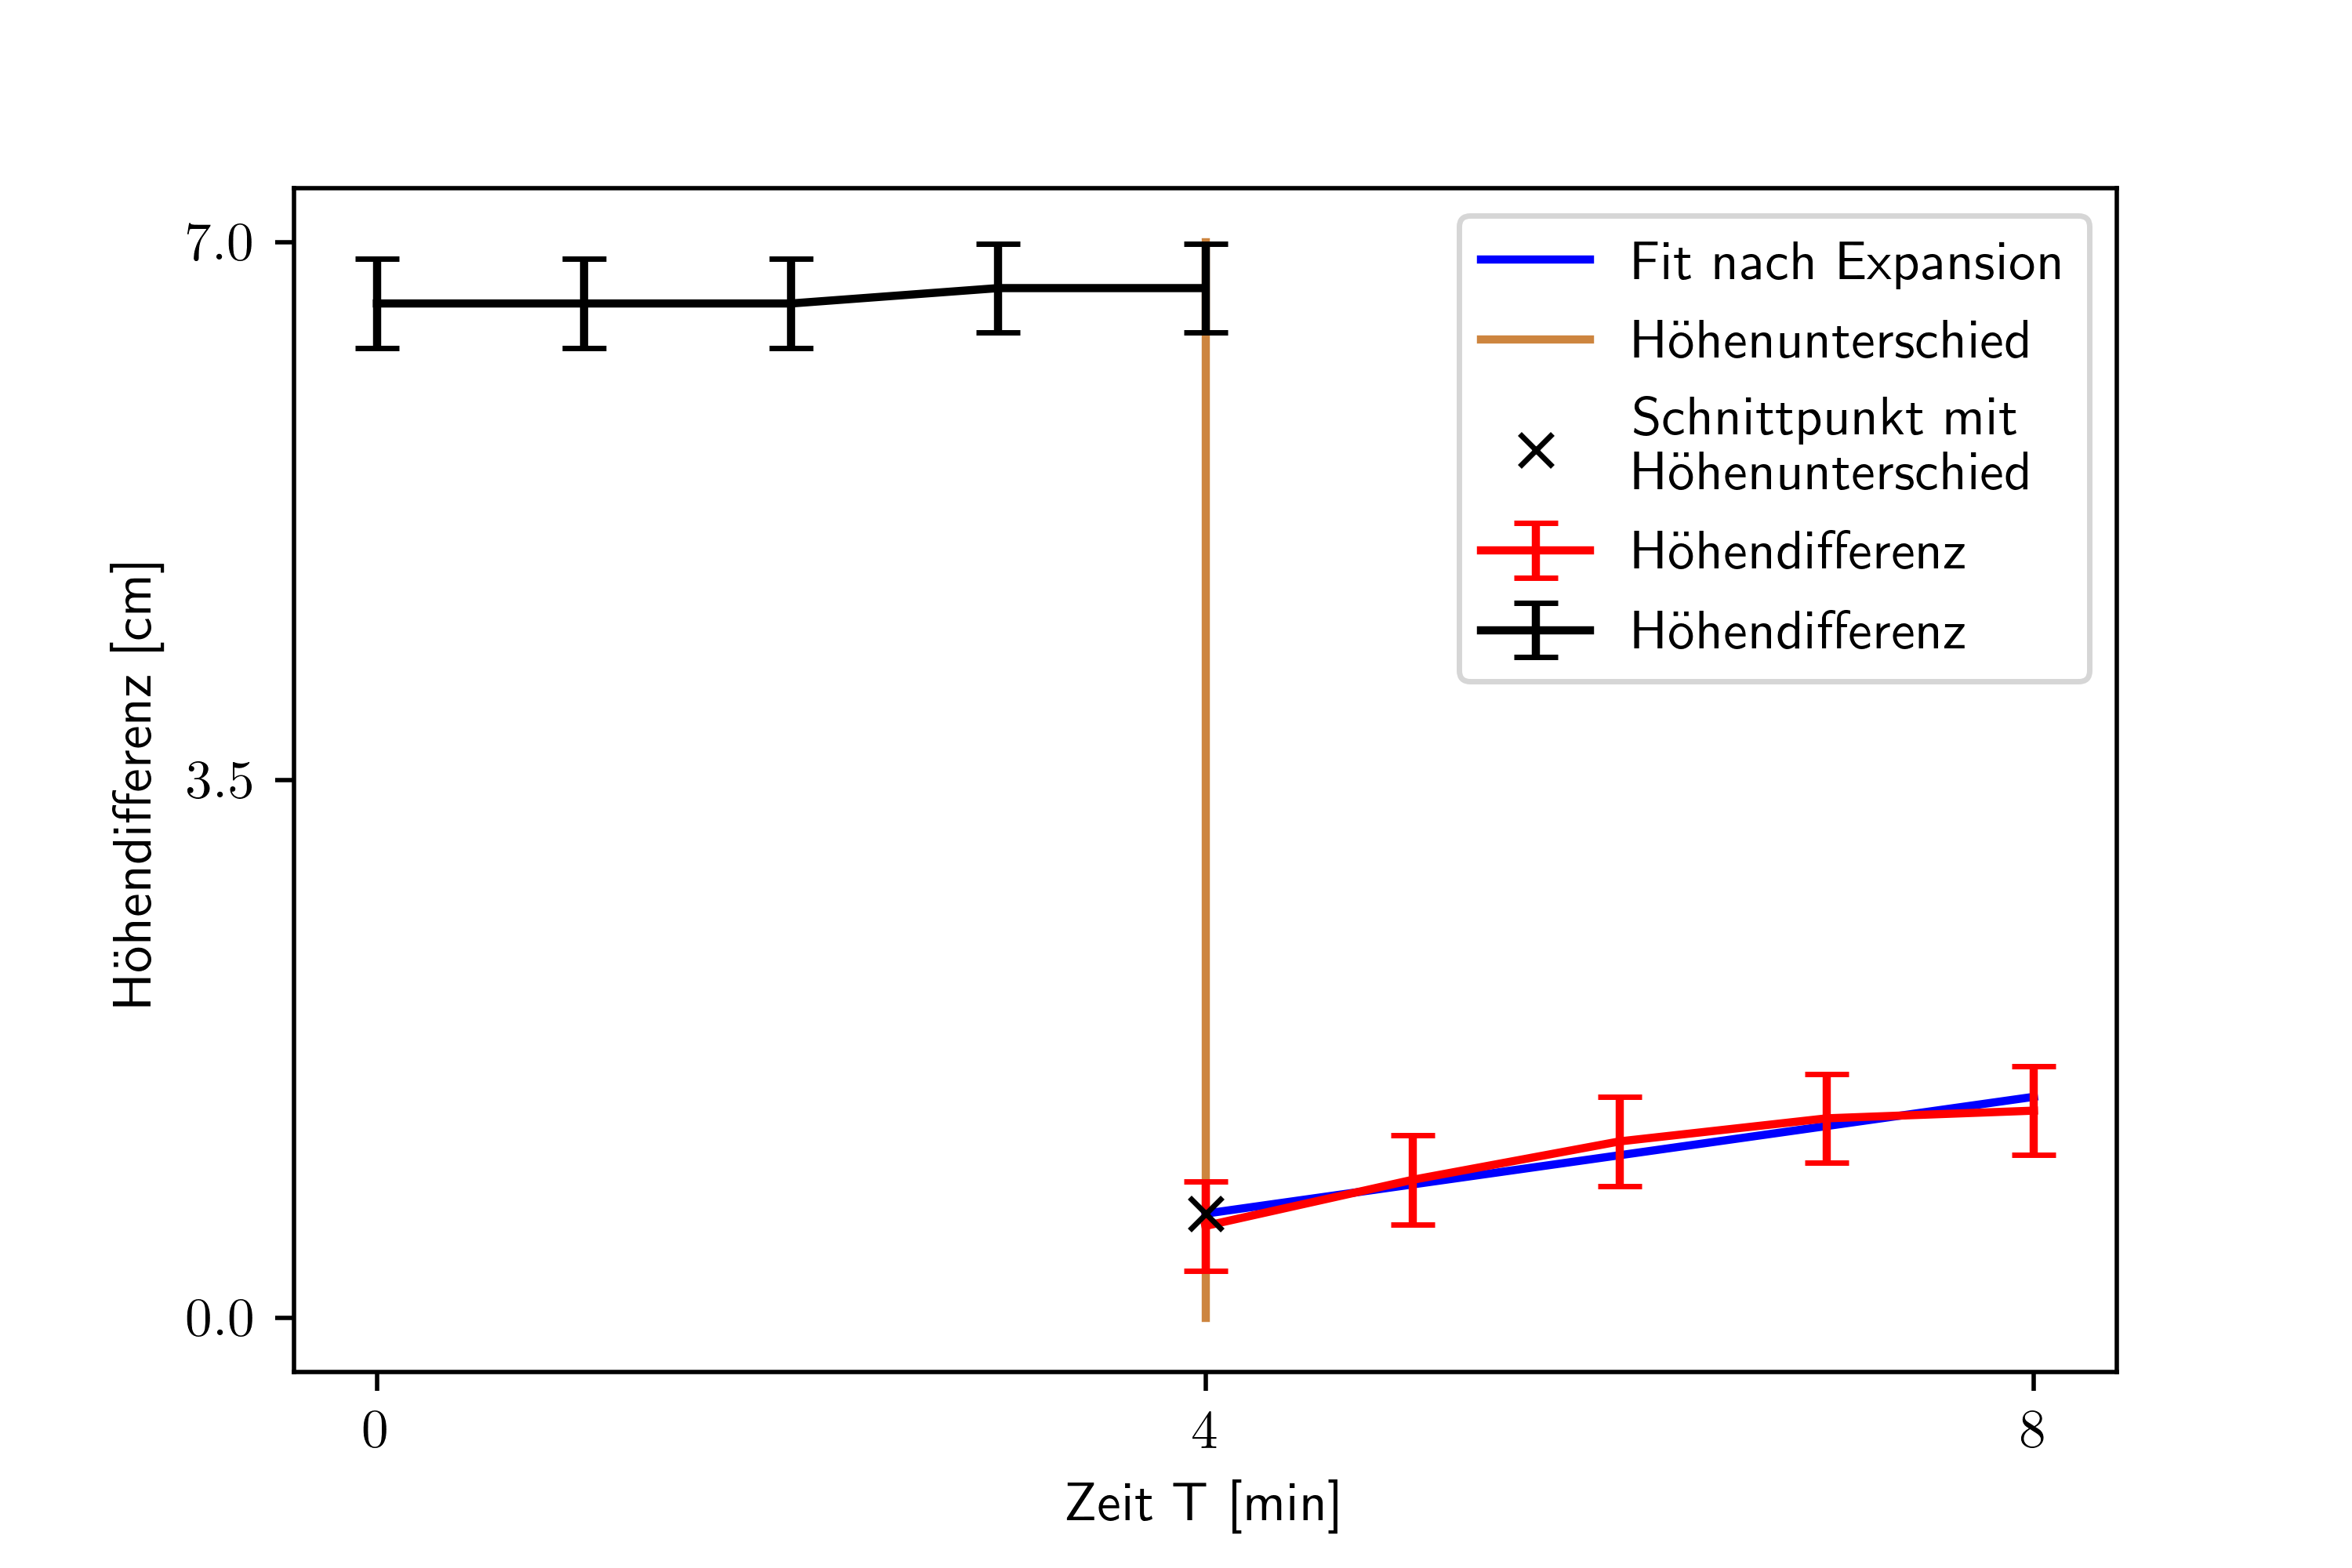
\includegraphics[width=350pt]{fotos/gpr1/Regression_M1.png}			% einfügen des Bildes/ mit width Bildbreite einstellen
		\caption{Messreihe 1, von \theauthor}							% Bildunterschrift
		\label{Abb: Ben 1}							% für Textverweise
	\end{figure}
\begin{figure}[!ht]
	\centering									% Bild Zentrierung
	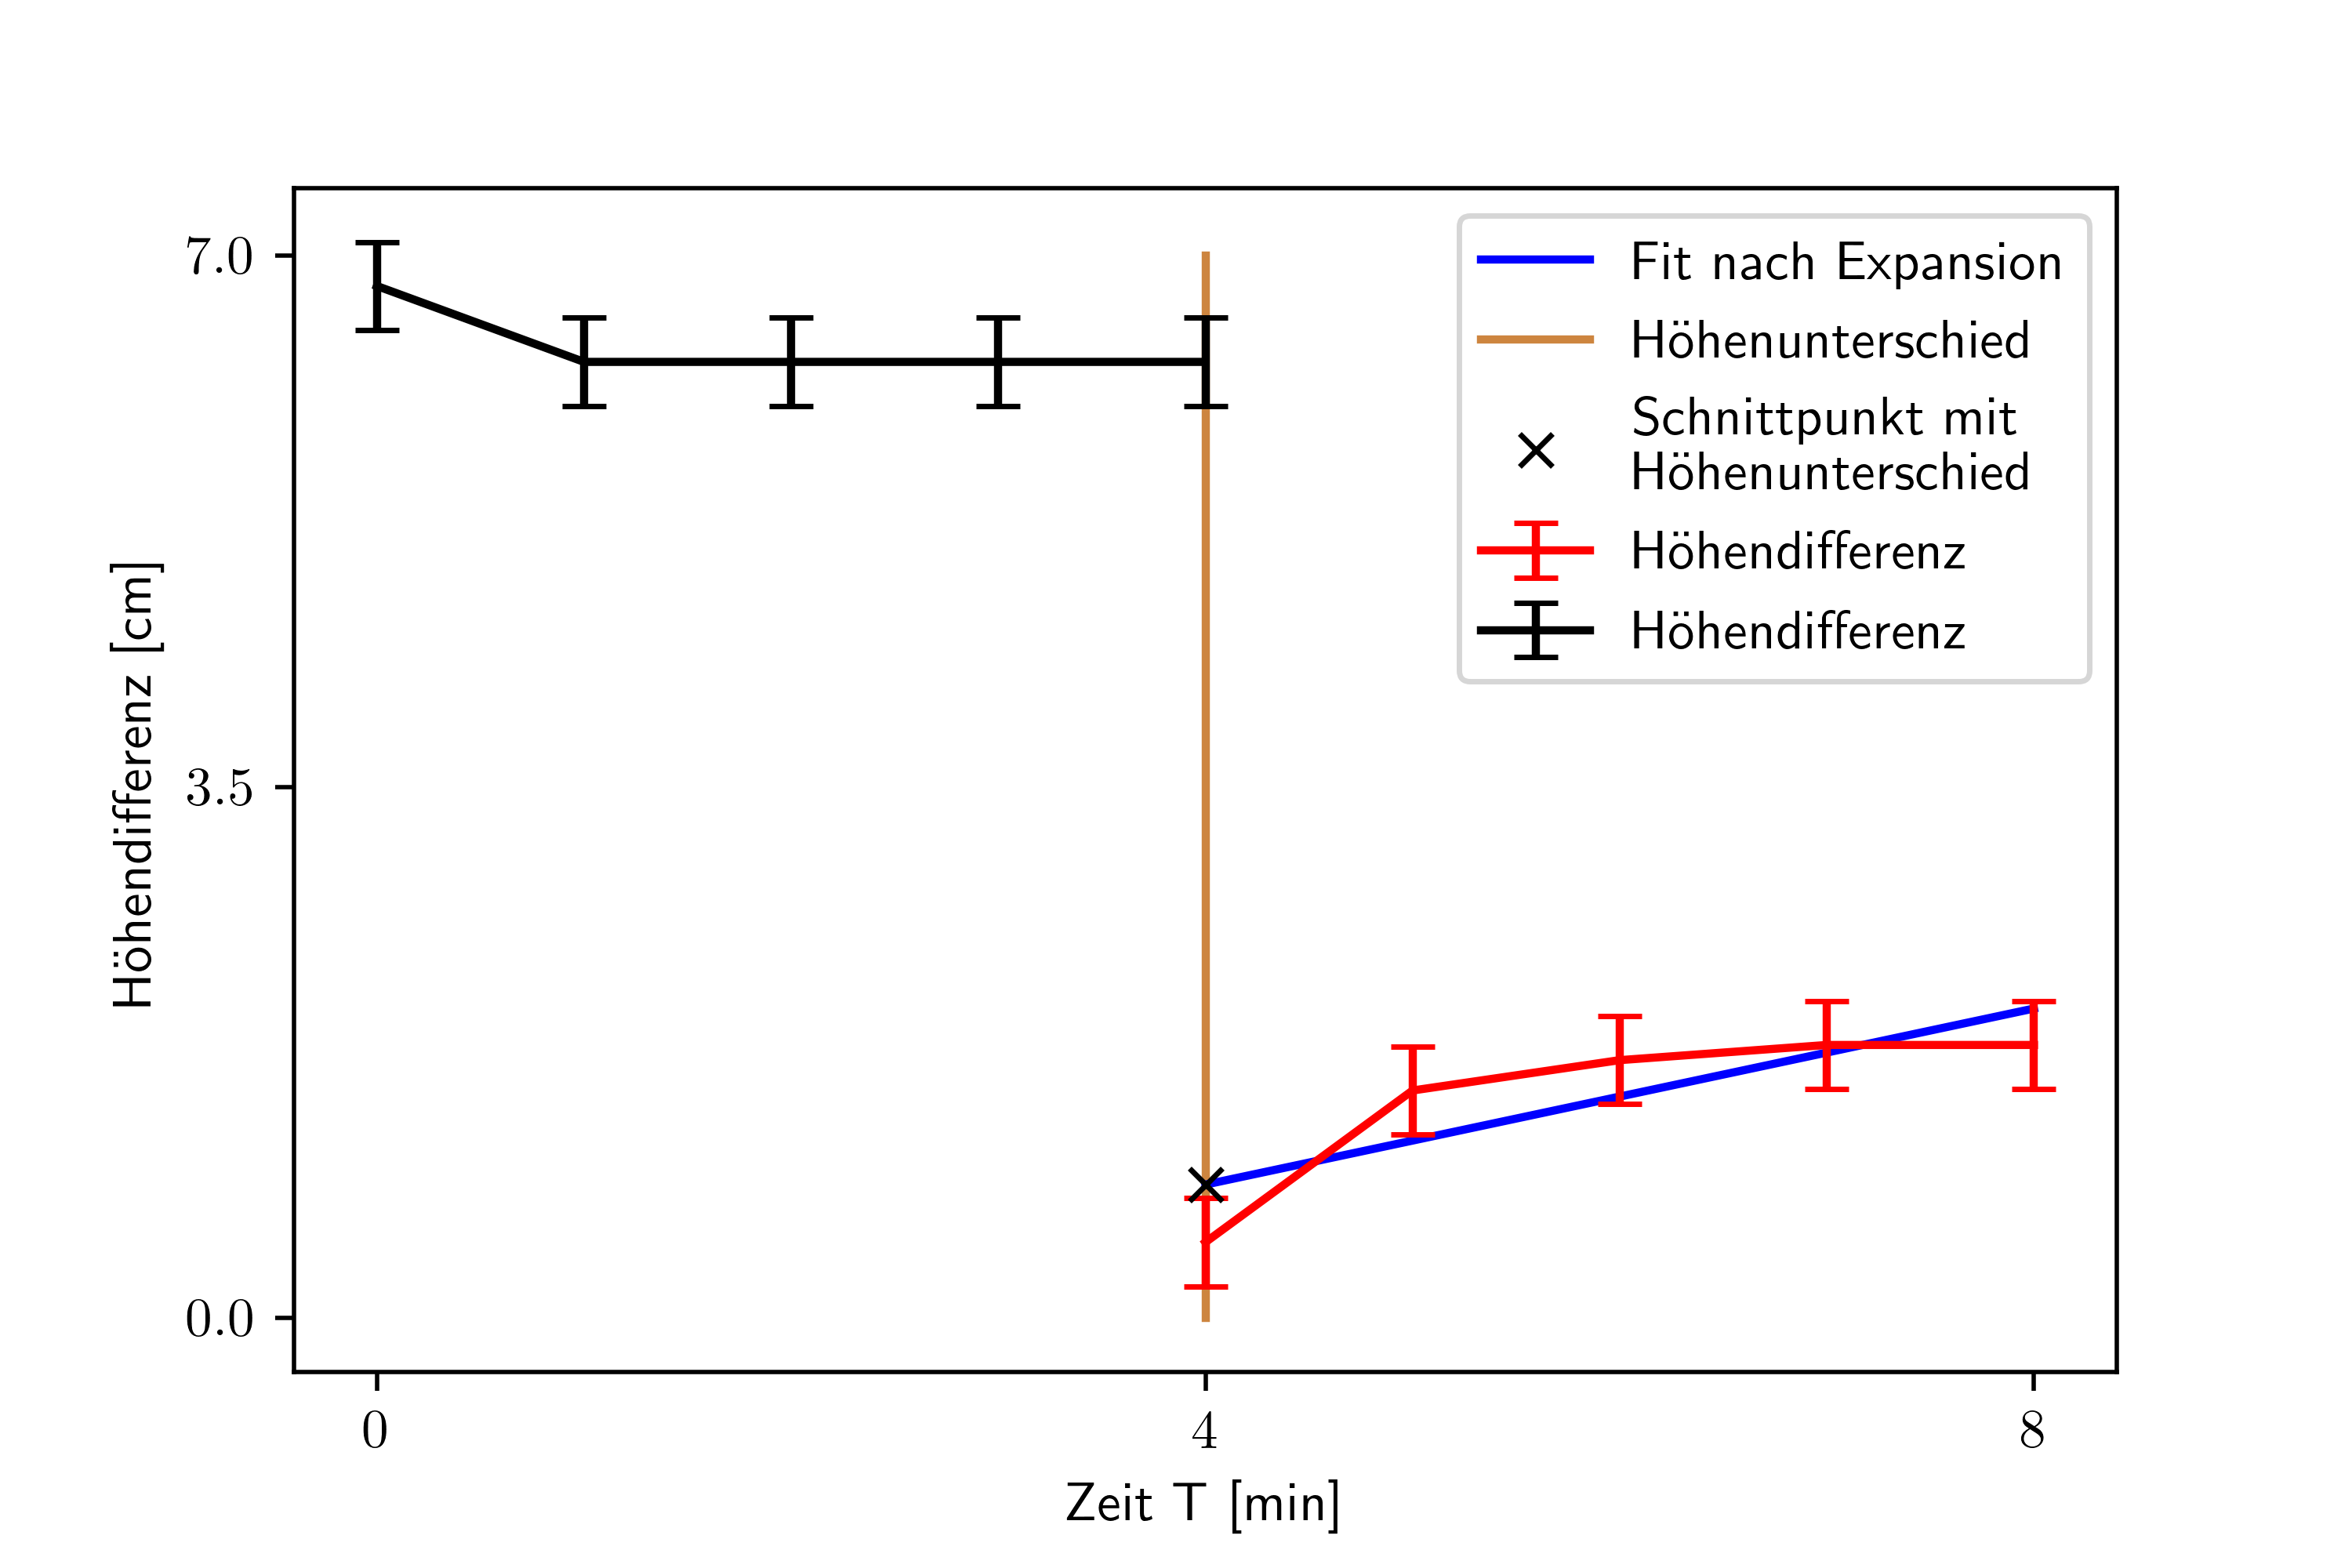
\includegraphics[width=350pt]{fotos/gpr1/Regression_M2.png}			% einfügen des Bildes/ mit width Bildbreite einstellen
	\caption{Messreihe 2, von \theauthor}							% Bildunterschrift
	\label{Abb: Ben 2}							% für Textverweise
\end{figure}
\newpage
\begin{figure}[!ht]
\centering									% Bild Zentrierung
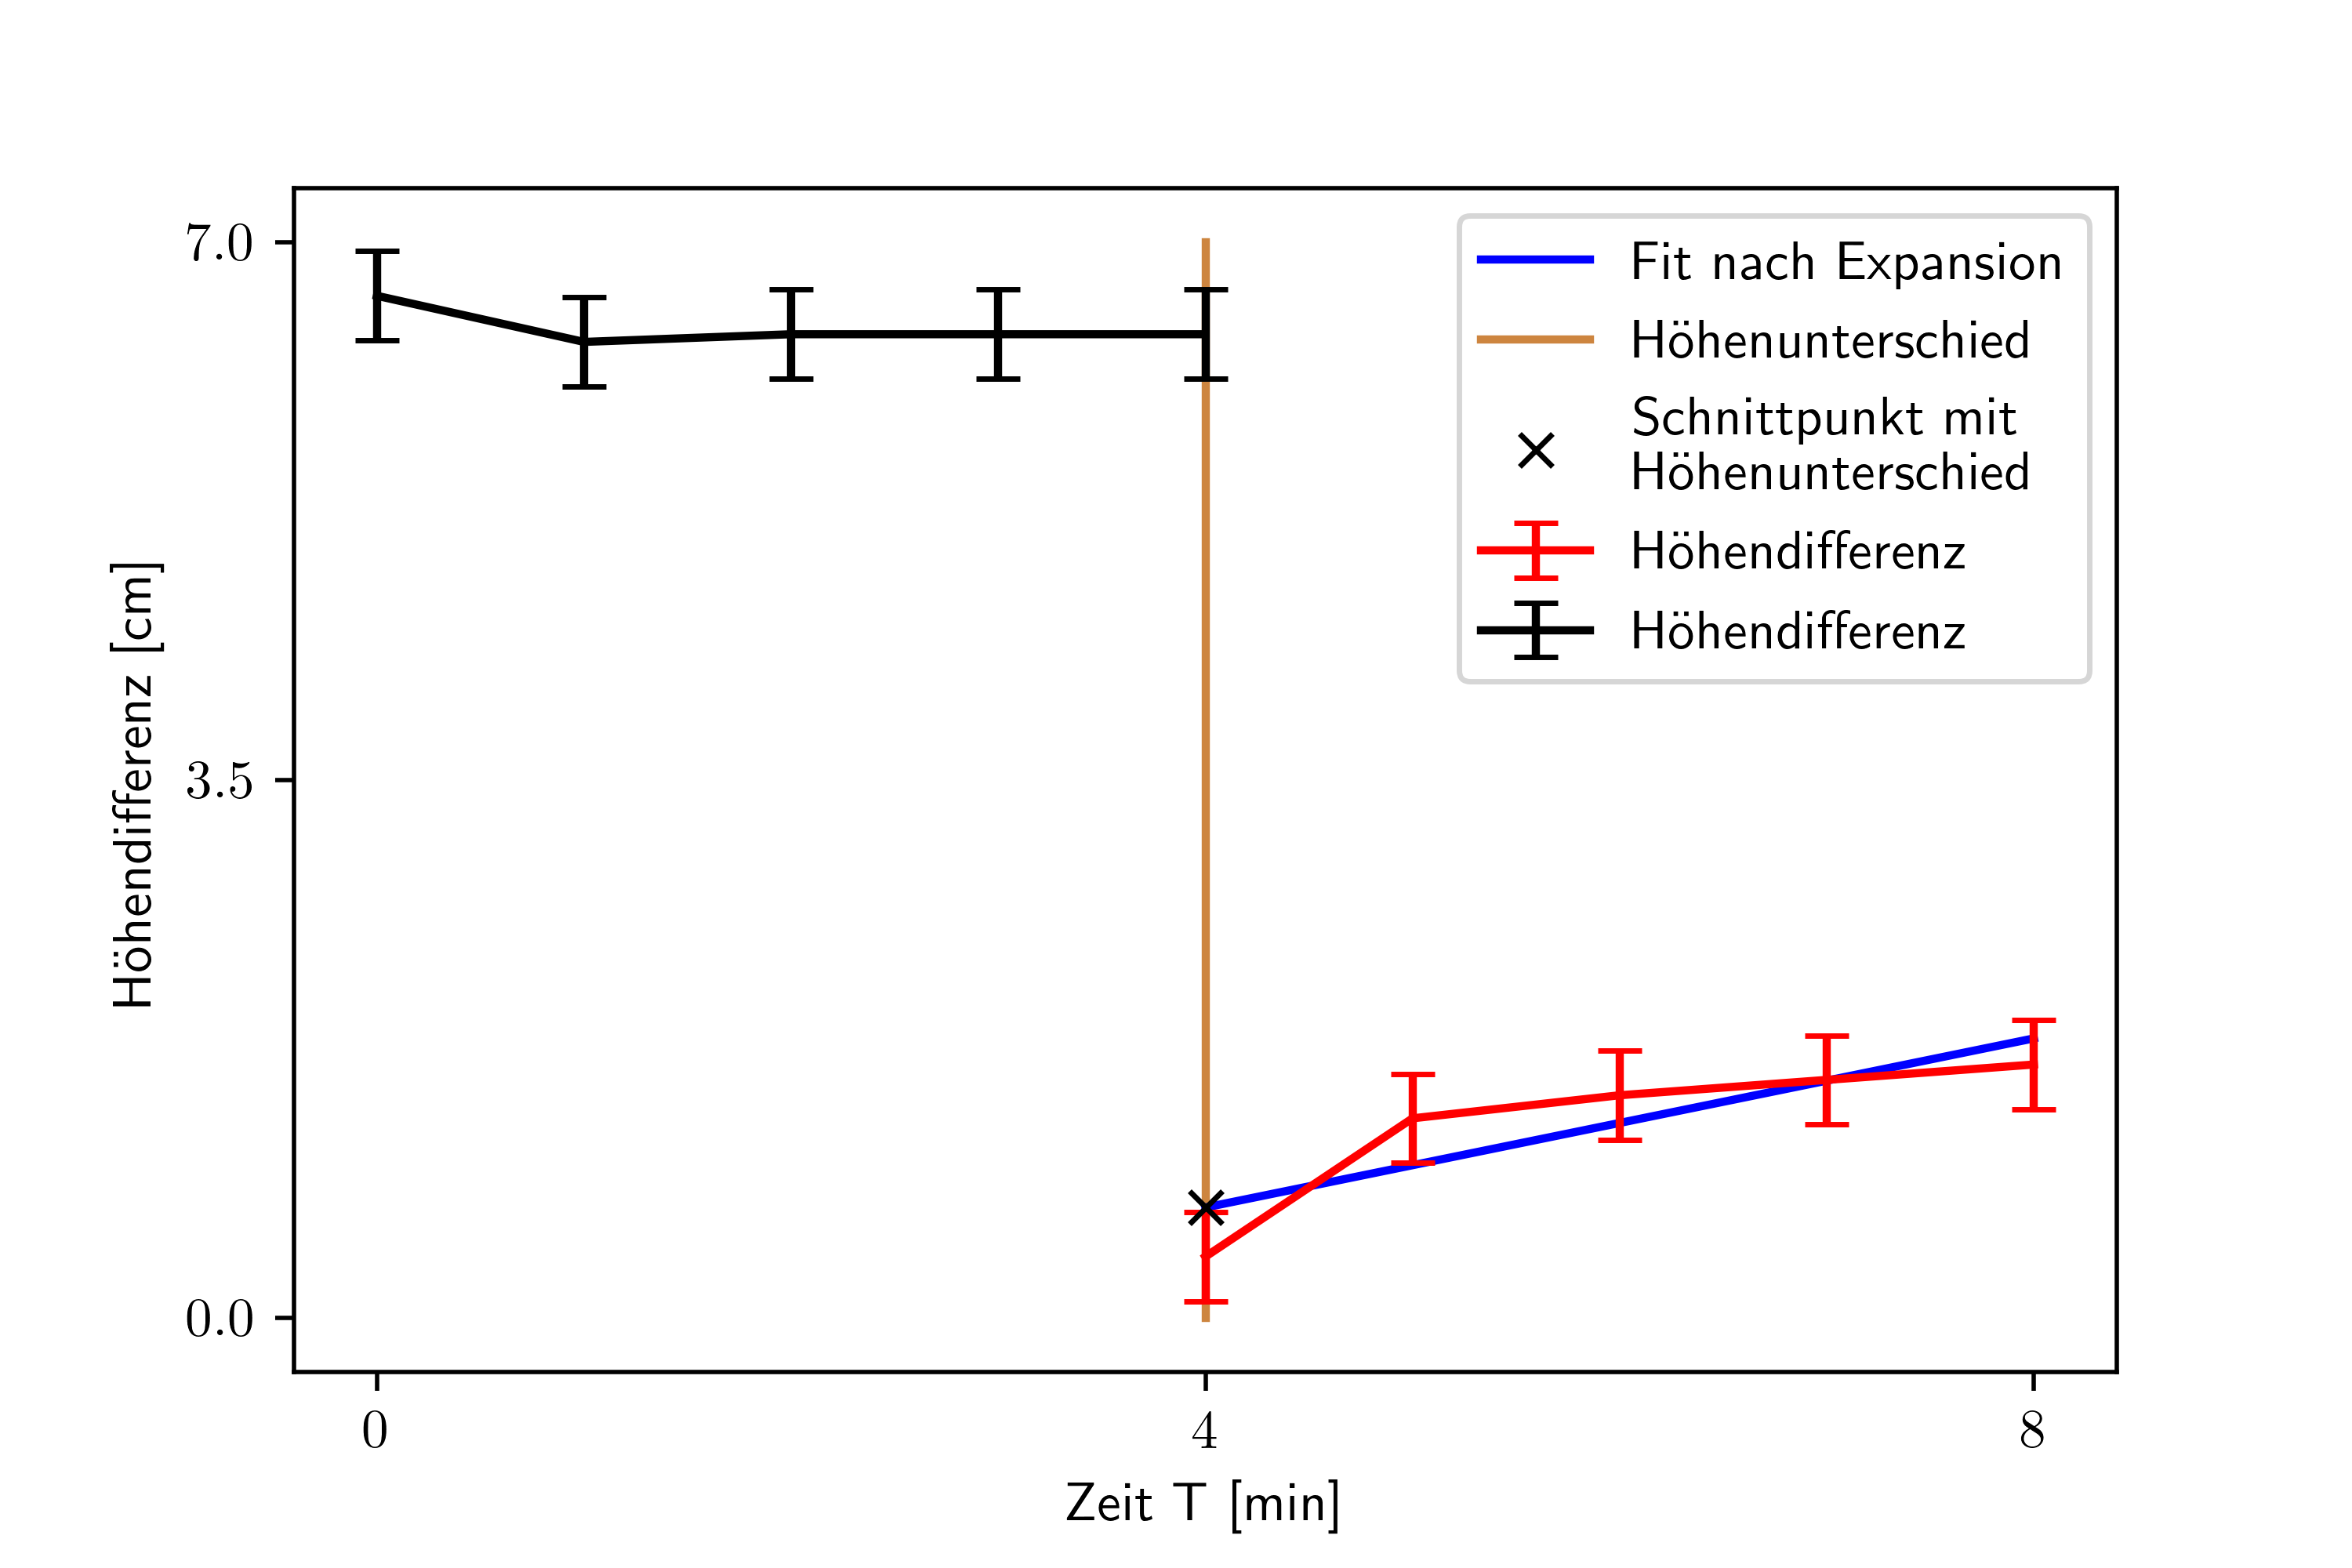
\includegraphics[width=350pt]{fotos/gpr1/Regression_M3.png}			% einfügen des Bildes/ mit width Bildbreite einstellen
\caption{Messreihe 3, von \theauthor}							% Bildunterschrift
\label{Abb: Ben 3}							% für Textverweise
\end{figure}
\begin{figure}[!ht]
\centering									% Bild Zentrierung
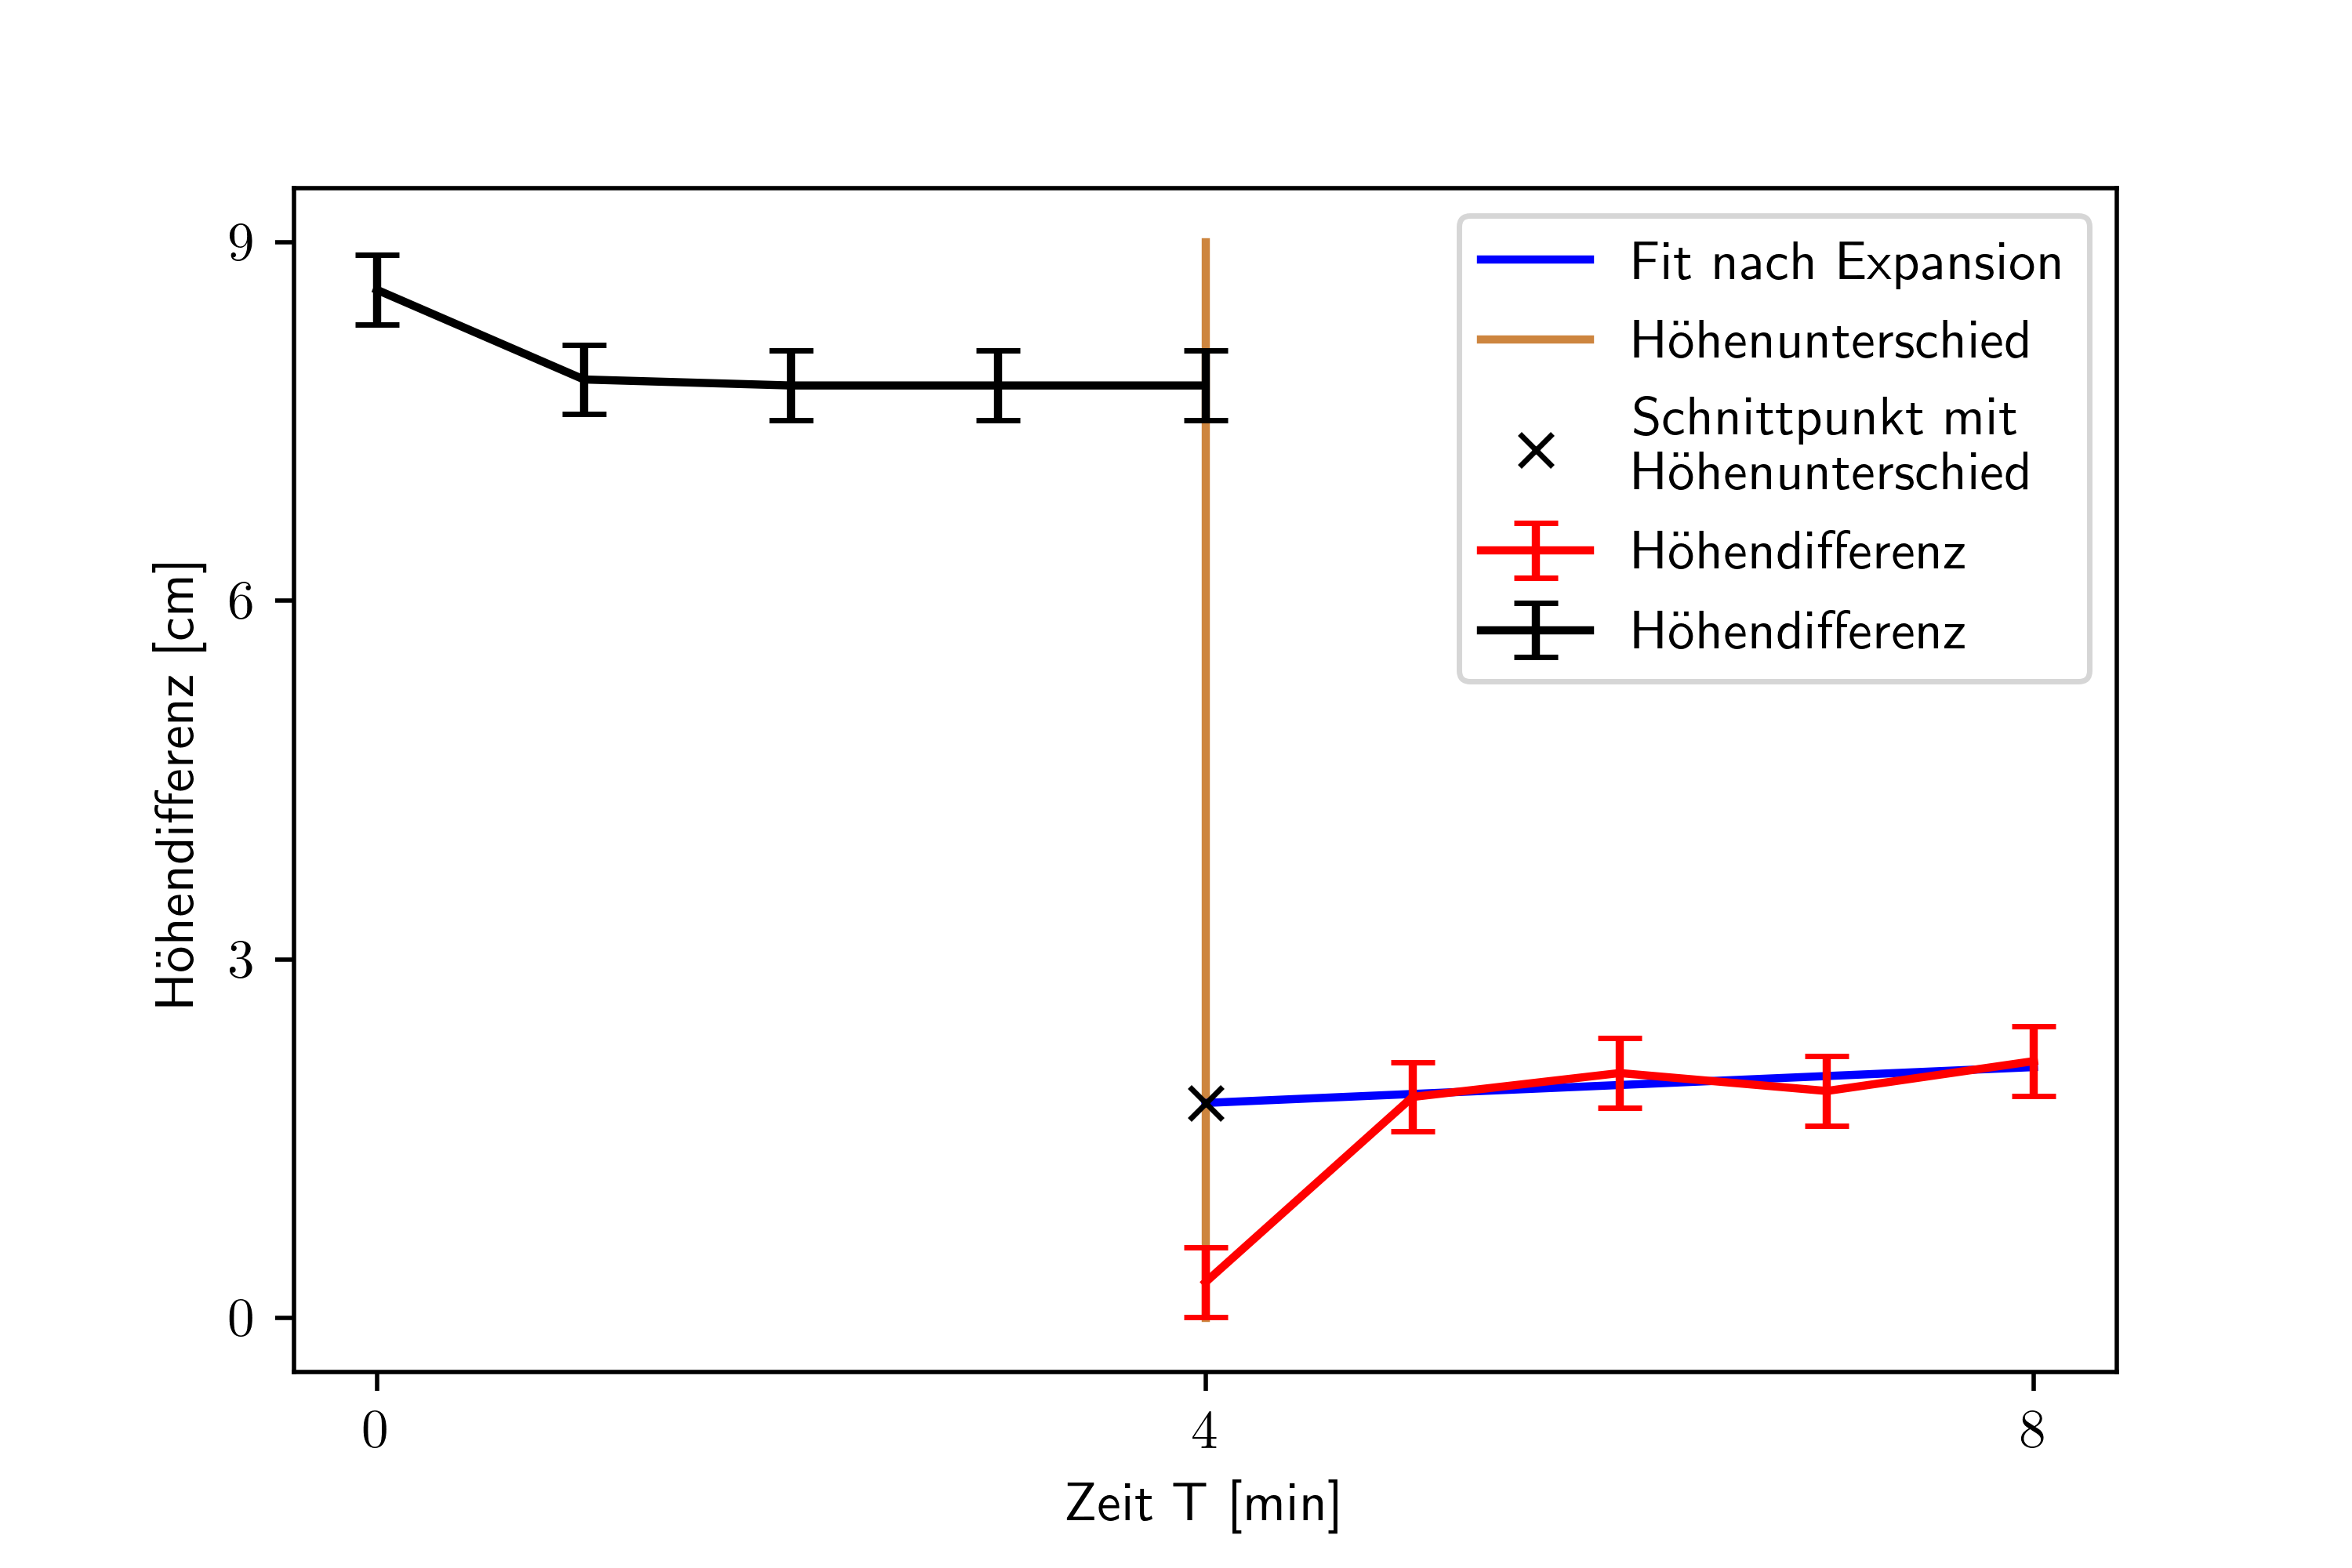
\includegraphics[width=350pt]{fotos/gpr1/Regression-M4.png}			% einfügen des Bildes/ mit width Bildbreite einstellen
\caption{Messreihe 4, von \theauthor}							% Bildunterschrift
\label{Abb: Ben 4}							% für Textverweise
\end{figure}
	\newpage
\begin{figure}[!ht]
	\centering									% Bild Zentrierung
	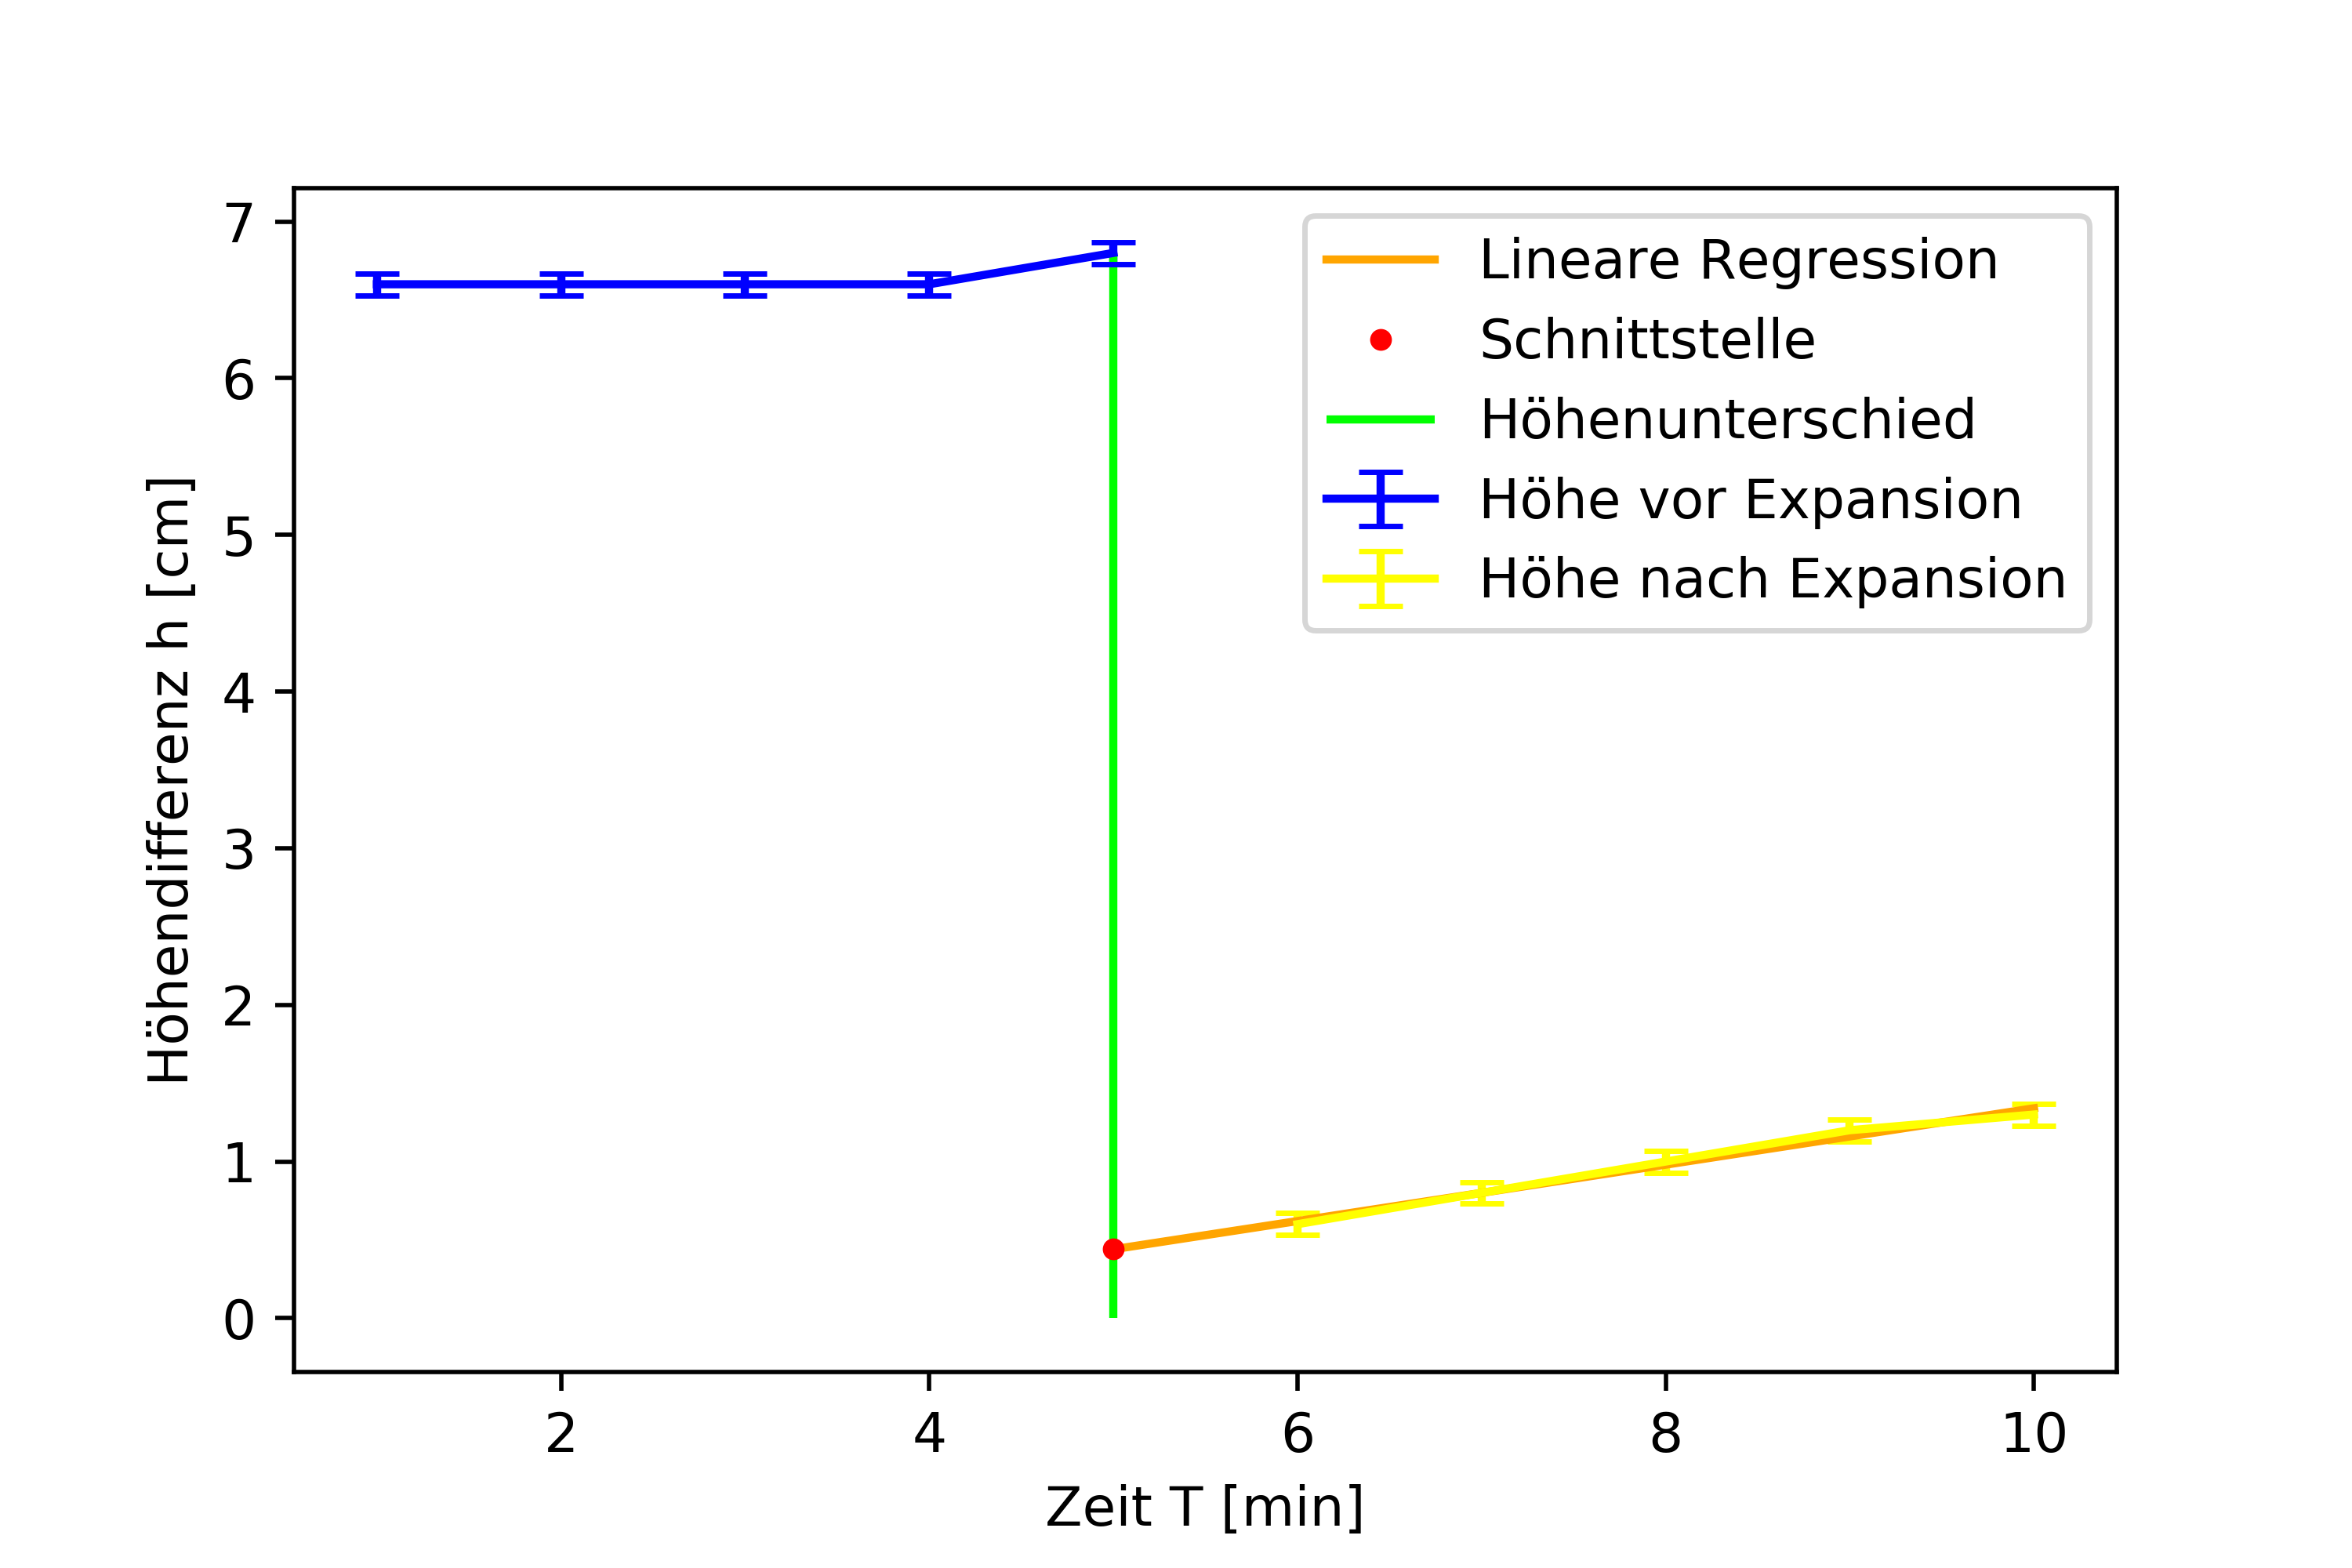
\includegraphics[width=400pt]{fotos/gpr1/Temperaturkorrektor 1. Messung.png}			% einfügen des Bildes/ mit width Bildbreite einstellen
	\caption{Messreihe 5}							% Bildunterschrift
	\label{Abb: Sara 1}							% für Textverweise
\end{figure}
\begin{figure}[!ht]
	\centering									% Bild Zentrierung
	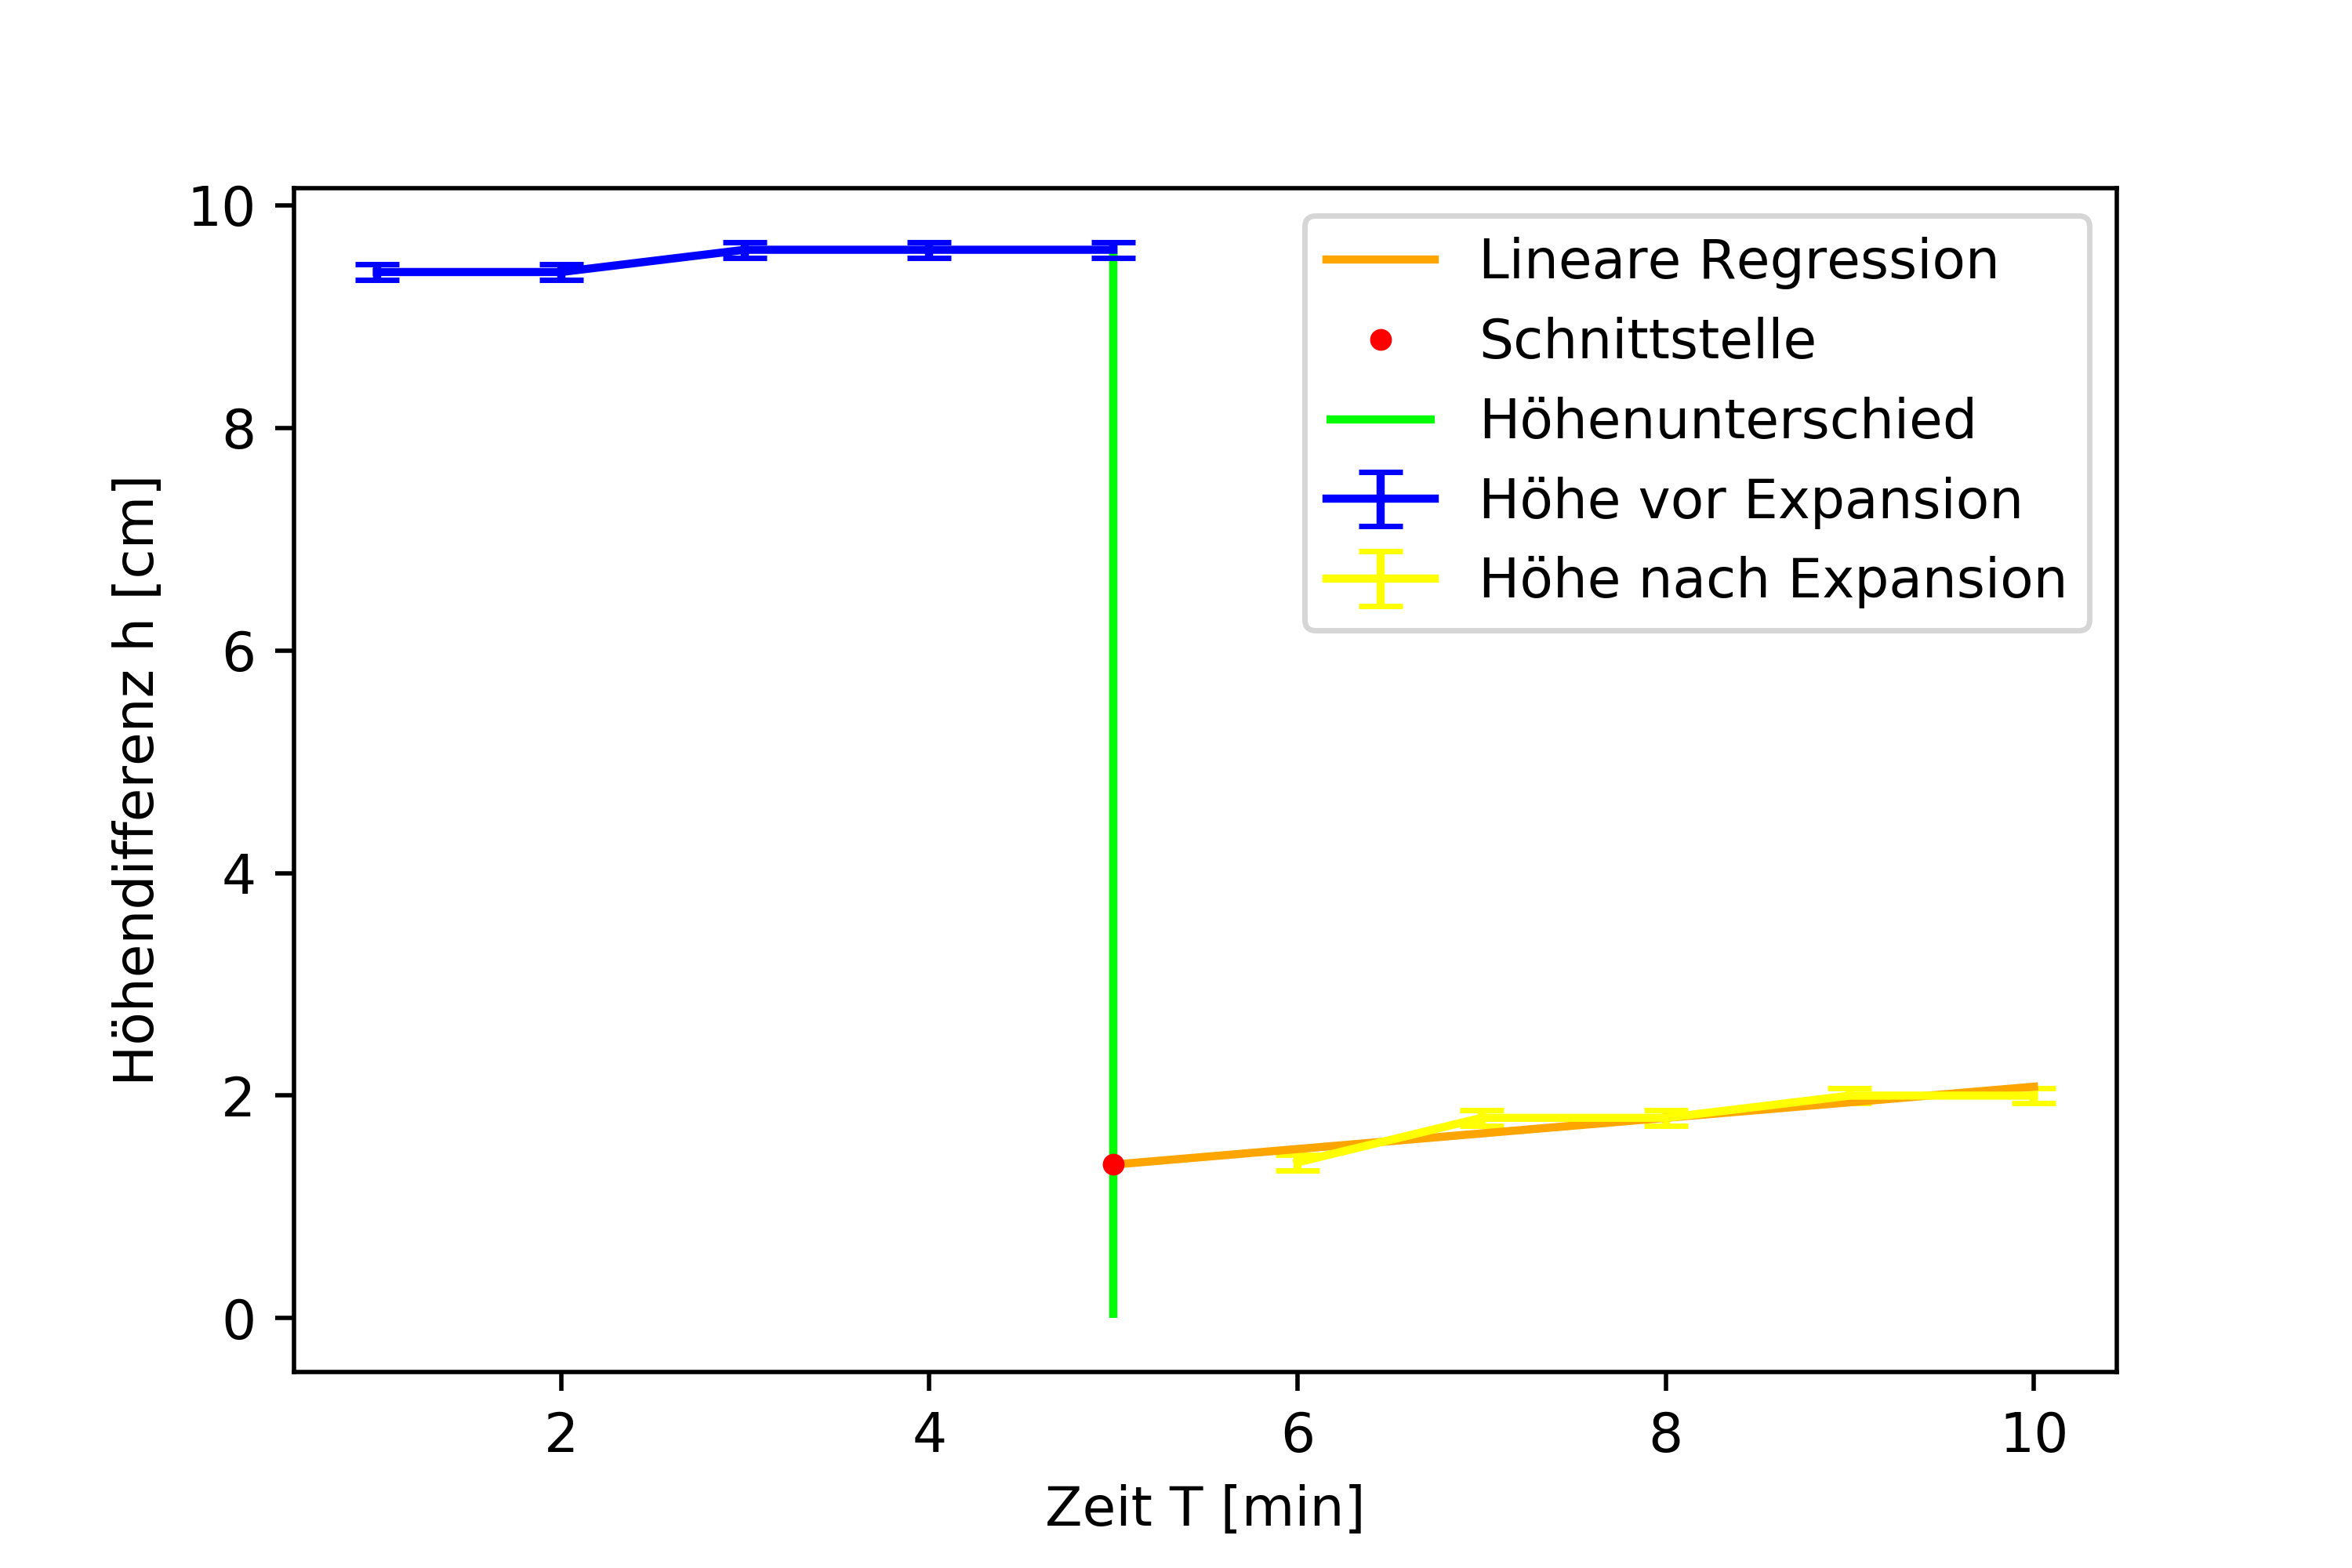
\includegraphics[width=400pt]{fotos/gpr1/Temperaturkorrektor 2. Messung.png}			% einfügen des Bildes/ mit width Bildbreite einstellen
	\caption{Messreihe 6}							% Bildunterschrift
	\label{Abb: Sara 2}							% für Textverweise
\end{figure}
\newpage
\begin{figure}[!ht]
	\centering									% Bild Zentrierung
	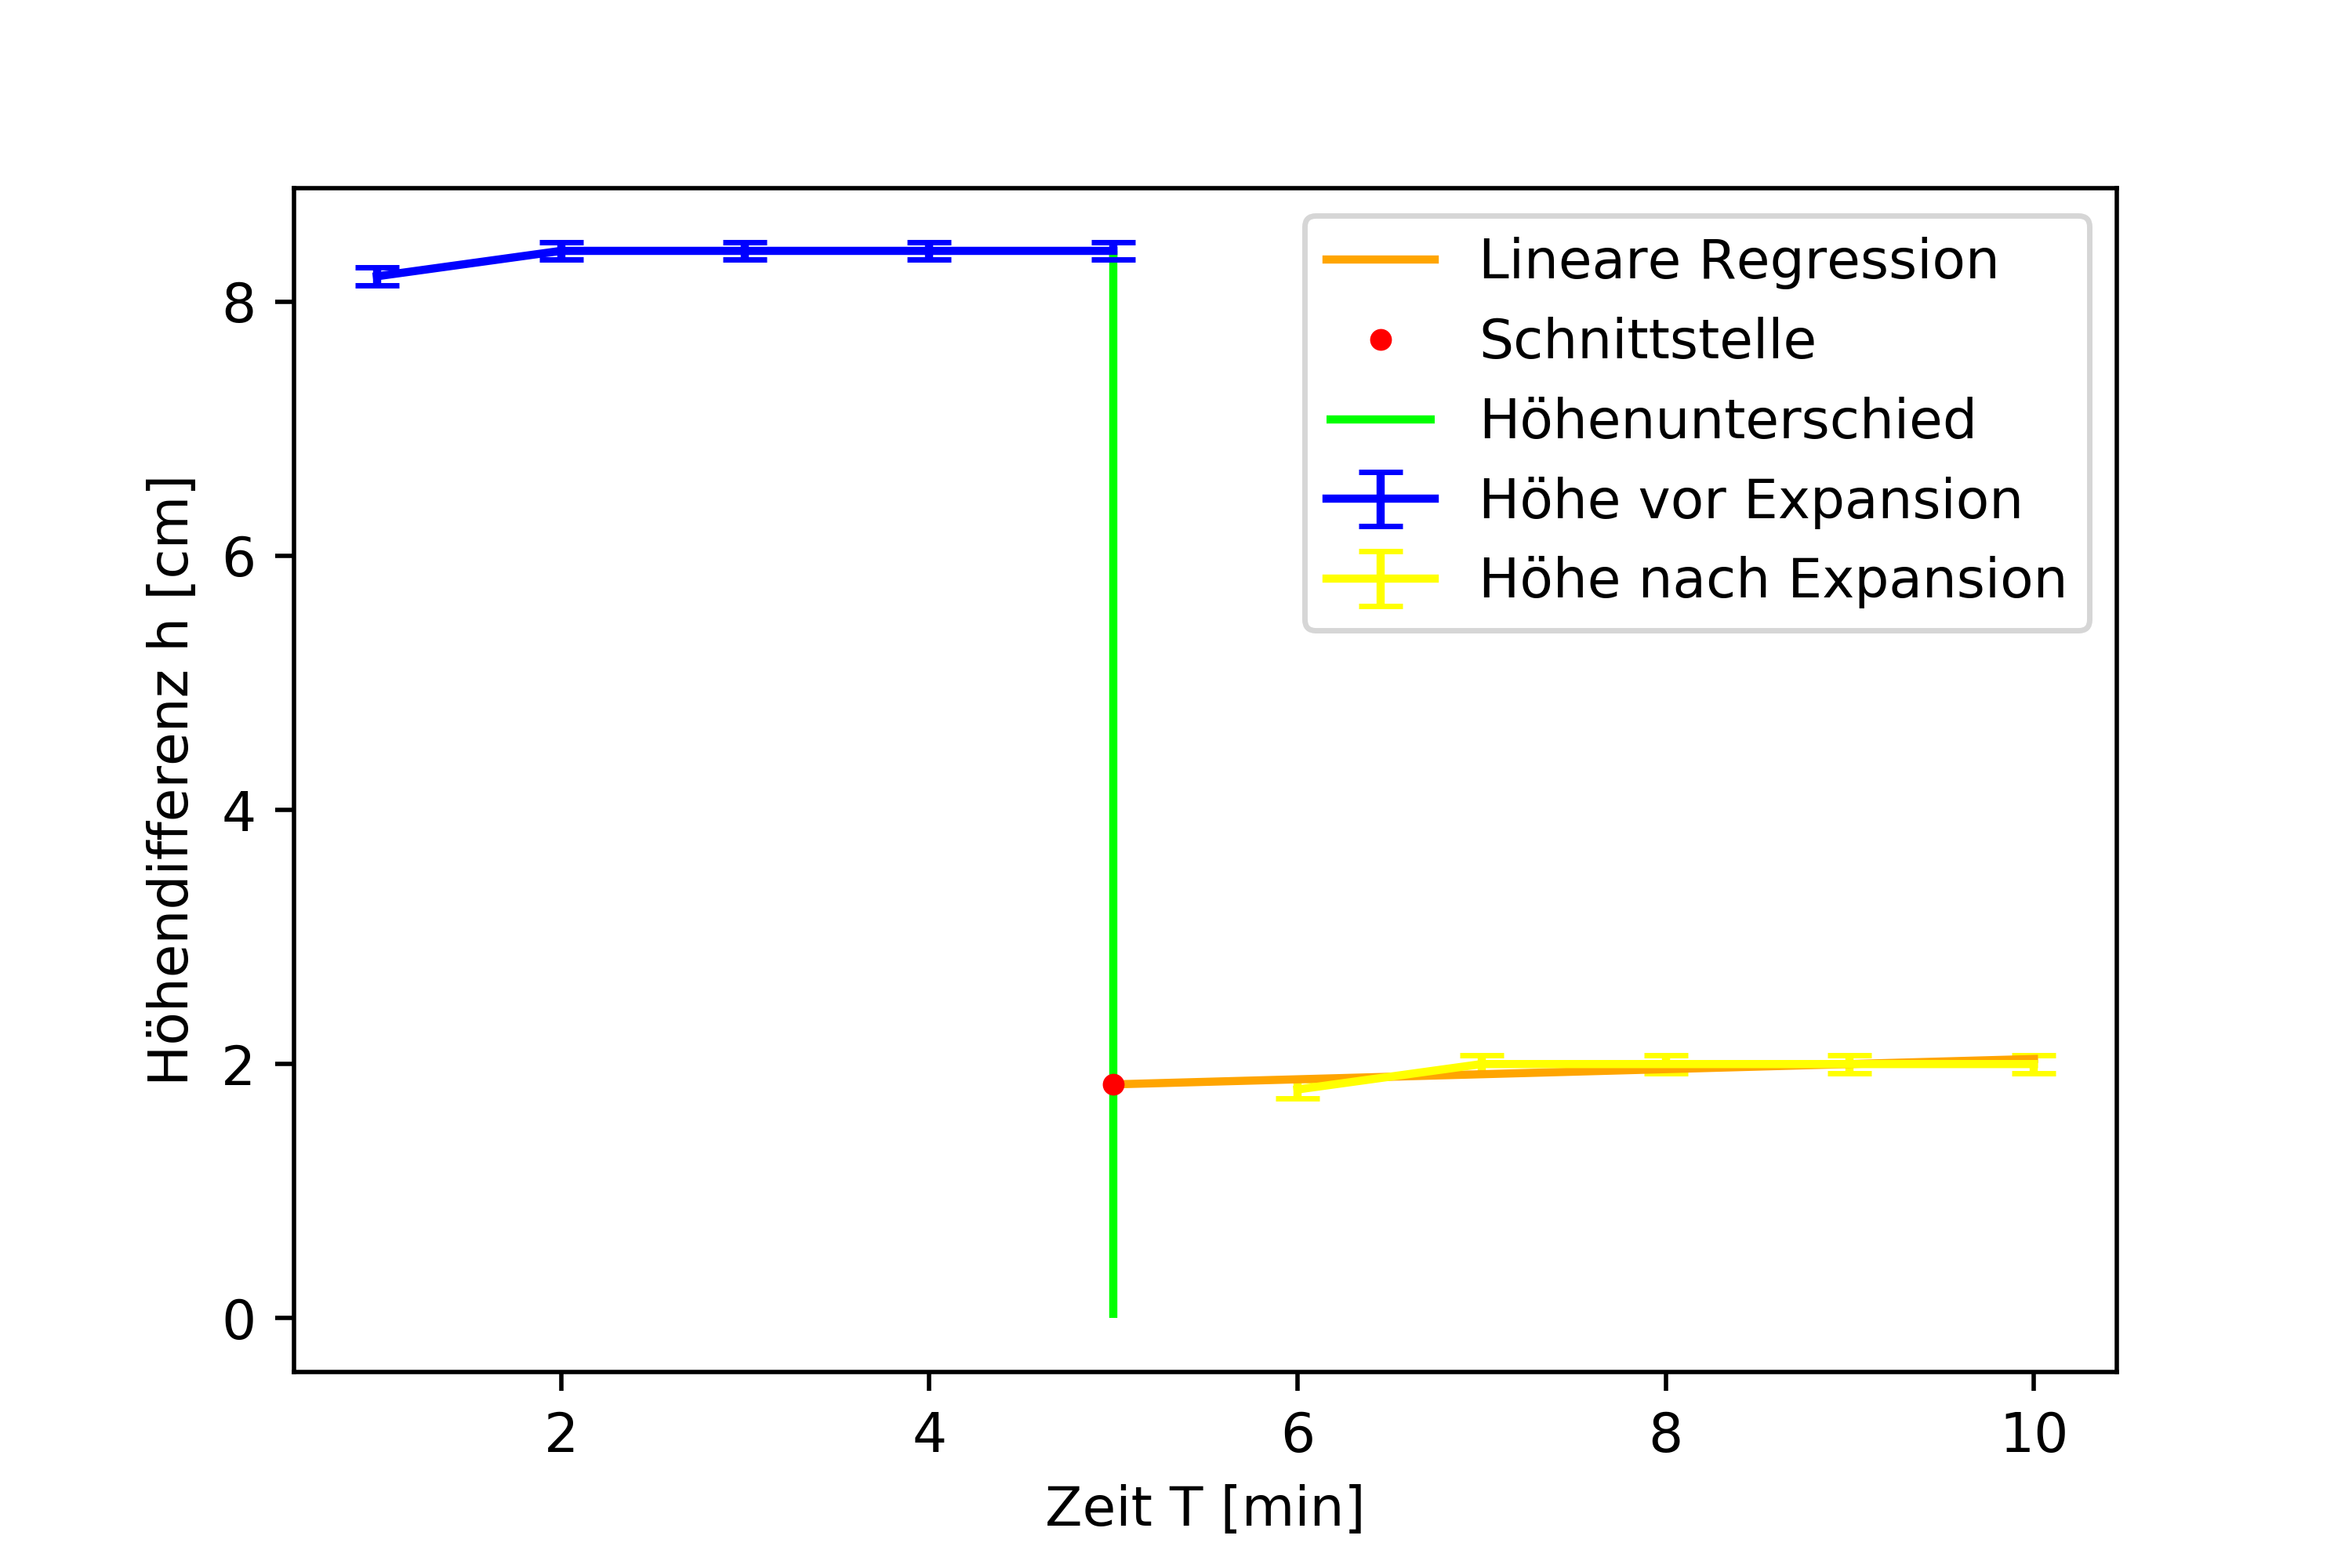
\includegraphics[width=400pt]{fotos/gpr1/Temperaturkorrektor 3. Messung.png}			% einfügen des Bildes/ mit width Bildbreite einstellen
	\caption{Messreihe 7}							% Bildunterschrift
	\label{Abb: Sara 3}							% für Textverweise
\end{figure}
\begin{figure}[!ht]
	\centering									% Bild Zentrierung
	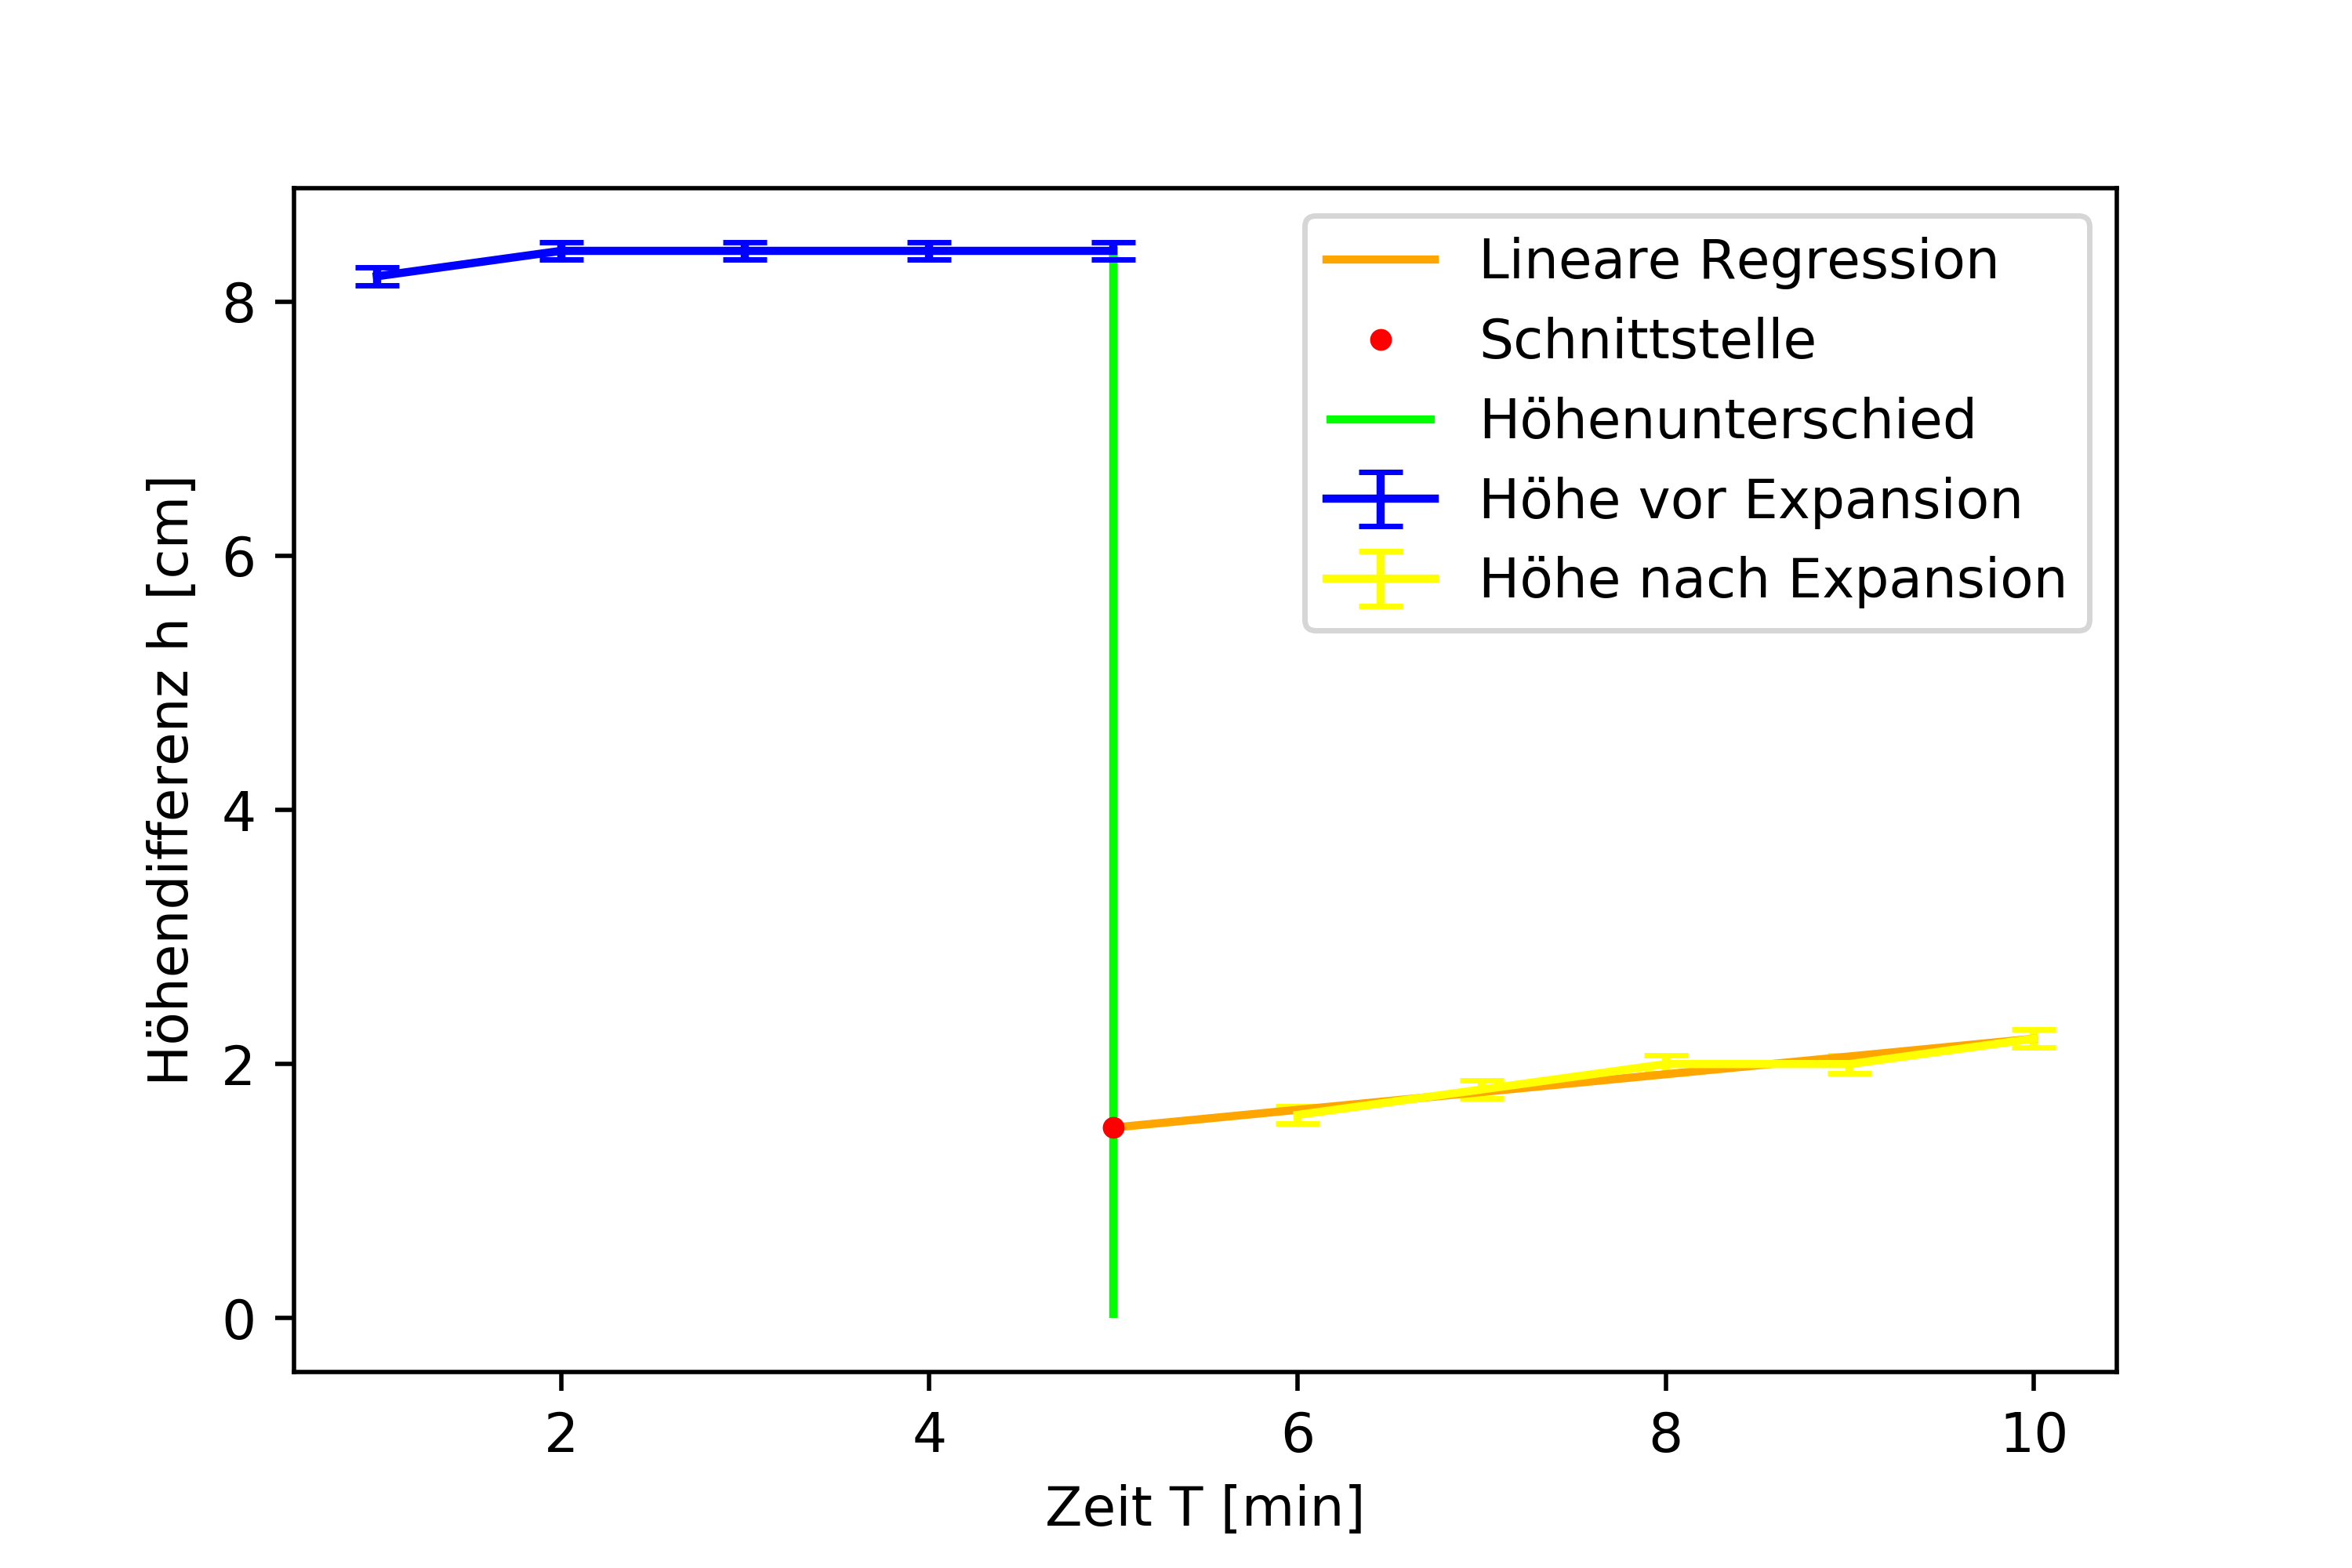
\includegraphics[width=400pt]{fotos/gpr1/Temperaturkorrektor 4. Messung.png}			% einfügen des Bildes/ mit width Bildbreite einstellen
	\caption{Messreihe 8}							% Bildunterschrift
	\label{Abb: Sara 4}							% für Textverweise
\end{figure}	
		
	

	\newpage
	\printbibliography[title={Quellenverzeichnis}]
	
	
\end{document}